\documentclass[twoside]{book}

% Packages required by doxygen
\usepackage{fixltx2e}
\usepackage{calc}
\usepackage{doxygen}
\usepackage[export]{adjustbox} % also loads graphicx
\usepackage{graphicx}
\usepackage[utf8]{inputenc}
\usepackage{makeidx}
\usepackage{multicol}
\usepackage{multirow}
\PassOptionsToPackage{warn}{textcomp}
\usepackage{textcomp}
\usepackage[nointegrals]{wasysym}
\usepackage[table]{xcolor}

% Font selection
\usepackage[T1]{fontenc}
\usepackage[scaled=.90]{helvet}
\usepackage{courier}
\usepackage{amssymb}
\usepackage{sectsty}
\renewcommand{\familydefault}{\sfdefault}
\allsectionsfont{%
  \fontseries{bc}\selectfont%
  \color{darkgray}%
}
\renewcommand{\DoxyLabelFont}{%
  \fontseries{bc}\selectfont%
  \color{darkgray}%
}
\newcommand{\+}{\discretionary{\mbox{\scriptsize$\hookleftarrow$}}{}{}}

% Page & text layout
\usepackage{geometry}
\geometry{%
  a4paper,%
  top=2.5cm,%
  bottom=2.5cm,%
  left=2.5cm,%
  right=2.5cm%
}
\tolerance=750
\hfuzz=15pt
\hbadness=750
\setlength{\emergencystretch}{15pt}
\setlength{\parindent}{0cm}
\setlength{\parskip}{3ex plus 2ex minus 2ex}
\makeatletter
\renewcommand{\paragraph}{%
  \@startsection{paragraph}{4}{0ex}{-1.0ex}{1.0ex}{%
    \normalfont\normalsize\bfseries\SS@parafont%
  }%
}
\renewcommand{\subparagraph}{%
  \@startsection{subparagraph}{5}{0ex}{-1.0ex}{1.0ex}{%
    \normalfont\normalsize\bfseries\SS@subparafont%
  }%
}
\makeatother

% Headers & footers
\usepackage{fancyhdr}
\pagestyle{fancyplain}
\fancyhead[LE]{\fancyplain{}{\bfseries\thepage}}
\fancyhead[CE]{\fancyplain{}{}}
\fancyhead[RE]{\fancyplain{}{\bfseries\leftmark}}
\fancyhead[LO]{\fancyplain{}{\bfseries\rightmark}}
\fancyhead[CO]{\fancyplain{}{}}
\fancyhead[RO]{\fancyplain{}{\bfseries\thepage}}
\fancyfoot[LE]{\fancyplain{}{}}
\fancyfoot[CE]{\fancyplain{}{}}
\fancyfoot[RE]{\fancyplain{}{\bfseries\scriptsize Generated by Doxygen }}
\fancyfoot[LO]{\fancyplain{}{\bfseries\scriptsize Generated by Doxygen }}
\fancyfoot[CO]{\fancyplain{}{}}
\fancyfoot[RO]{\fancyplain{}{}}
\renewcommand{\footrulewidth}{0.4pt}
\renewcommand{\chaptermark}[1]{%
  \markboth{#1}{}%
}
\renewcommand{\sectionmark}[1]{%
  \markright{\thesection\ #1}%
}

% Indices & bibliography
\usepackage{natbib}
\usepackage[titles]{tocloft}
\setcounter{tocdepth}{3}
\setcounter{secnumdepth}{5}
\makeindex

% Hyperlinks (required, but should be loaded last)
\usepackage{ifpdf}
\ifpdf
  \usepackage[pdftex,pagebackref=true]{hyperref}
\else
  \usepackage[ps2pdf,pagebackref=true]{hyperref}
\fi
\hypersetup{%
  colorlinks=true,%
  linkcolor=blue,%
  citecolor=blue,%
  unicode%
}

% Custom commands
\newcommand{\clearemptydoublepage}{%
  \newpage{\pagestyle{empty}\cleardoublepage}%
}

\usepackage{caption}
\captionsetup{labelsep=space,justification=centering,font={bf},singlelinecheck=off,skip=4pt,position=top}

%===== C O N T E N T S =====

\begin{document}

% Titlepage & ToC
\hypersetup{pageanchor=false,
             bookmarksnumbered=true,
             pdfencoding=unicode
            }
\pagenumbering{alph}
\begin{titlepage}
\vspace*{7cm}
\begin{center}%
{\Large Ray Tracer \\[1ex]\large 1.\+0 }\\
\vspace*{1cm}
{\large Generated by Doxygen 1.8.14}\\
\end{center}
\end{titlepage}
\clearemptydoublepage
\pagenumbering{roman}
\tableofcontents
\clearemptydoublepage
\pagenumbering{arabic}
\hypersetup{pageanchor=true}

%--- Begin generated contents ---
\chapter{Hierarchical Index}
\section{Class Hierarchy}
This inheritance list is sorted roughly, but not completely, alphabetically\+:\begin{DoxyCompactList}
\item \contentsline{section}{Camera}{\pageref{class_camera}}{}
\item \contentsline{section}{Intersect}{\pageref{struct_intersect}}{}
\item \contentsline{section}{Light}{\pageref{class_light}}{}
\item \contentsline{section}{Object}{\pageref{class_object}}{}
\begin{DoxyCompactList}
\item \contentsline{section}{Plane}{\pageref{class_plane}}{}
\item \contentsline{section}{Sphere}{\pageref{class_sphere}}{}
\end{DoxyCompactList}
\item \contentsline{section}{Ray}{\pageref{struct_ray}}{}
\end{DoxyCompactList}

\chapter{Class Index}
\section{Class List}
Here are the classes, structs, unions and interfaces with brief descriptions\+:\begin{DoxyCompactList}
\item\contentsline{section}{\mbox{\hyperlink{class_camera}{Camera}} }{\pageref{class_camera}}{}
\item\contentsline{section}{\mbox{\hyperlink{struct_intersect}{Intersect}} \\*An tracks the point of intersection }{\pageref{struct_intersect}}{}
\item\contentsline{section}{\mbox{\hyperlink{class_light}{Light}} }{\pageref{class_light}}{}
\item\contentsline{section}{\mbox{\hyperlink{class_object}{Object}} }{\pageref{class_object}}{}
\item\contentsline{section}{\mbox{\hyperlink{class_plane}{Plane}} }{\pageref{class_plane}}{}
\item\contentsline{section}{\mbox{\hyperlink{struct_ray}{Ray}} \\*A \mbox{\hyperlink{struct_ray}{Ray}} that can be fired from things }{\pageref{struct_ray}}{}
\item\contentsline{section}{\mbox{\hyperlink{class_sphere}{Sphere}} }{\pageref{class_sphere}}{}
\end{DoxyCompactList}

\chapter{File Index}
\section{File List}
Here is a list of all files with brief descriptions\+:\begin{DoxyCompactList}
\item\contentsline{section}{\mbox{\hyperlink{camera_8cpp}{camera.\+cpp}} }{\pageref{camera_8cpp}}{}
\item\contentsline{section}{\mbox{\hyperlink{camera_8h}{camera.\+h}} \\*The header for the camera class }{\pageref{camera_8h}}{}
\item\contentsline{section}{\mbox{\hyperlink{libs_8h}{libs.\+h}} \\*The header for external libraries that are used everywhere. Also defines T\+\_\+\+B\+I\+AS which helps with acne }{\pageref{libs_8h}}{}
\item\contentsline{section}{\mbox{\hyperlink{light_8cpp}{light.\+cpp}} }{\pageref{light_8cpp}}{}
\item\contentsline{section}{\mbox{\hyperlink{light_8h}{light.\+h}} \\*The header for the light class }{\pageref{light_8h}}{}
\item\contentsline{section}{\mbox{\hyperlink{main_8cpp}{main.\+cpp}} }{\pageref{main_8cpp}}{}
\item\contentsline{section}{\mbox{\hyperlink{object_8h}{object.\+h}} \\*The header for the object class }{\pageref{object_8h}}{}
\item\contentsline{section}{\mbox{\hyperlink{plane_8cpp}{plane.\+cpp}} }{\pageref{plane_8cpp}}{}
\item\contentsline{section}{\mbox{\hyperlink{plane_8h}{plane.\+h}} \\*The header for the plane class }{\pageref{plane_8h}}{}
\item\contentsline{section}{\mbox{\hyperlink{sceneload_8cpp}{sceneload.\+cpp}} }{\pageref{sceneload_8cpp}}{}
\item\contentsline{section}{\mbox{\hyperlink{sceneload_8h}{sceneload.\+h}} \\*The scene loader. This version assumes a vec3 setup }{\pageref{sceneload_8h}}{}
\item\contentsline{section}{\mbox{\hyperlink{sphere_8cpp}{sphere.\+cpp}} }{\pageref{sphere_8cpp}}{}
\item\contentsline{section}{\mbox{\hyperlink{sphere_8h}{sphere.\+h}} \\*The header for the sphere class }{\pageref{sphere_8h}}{}
\item\contentsline{section}{\mbox{\hyperlink{structs_8h}{structs.\+h}} \\*Home to the structs }{\pageref{structs_8h}}{}
\item\contentsline{section}{\mbox{\hyperlink{util_8cpp}{util.\+cpp}} }{\pageref{util_8cpp}}{}
\item\contentsline{section}{\mbox{\hyperlink{util_8h}{util.\+h}} \\*Header file for functions without a home. These get used by the program, but don\textquotesingle{}t belong to any particular class }{\pageref{util_8h}}{}
\end{DoxyCompactList}

\chapter{Class Documentation}
\hypertarget{class_camera}{}\section{Camera Class Reference}
\label{class_camera}\index{Camera@{Camera}}


\mbox{\hyperlink{class_camera}{Camera}} stores all of the camera related informaion. This class is loaded first and defies all of the scene related info.  




{\ttfamily \#include $<$camera.\+h$>$}

\subsection*{Public Member Functions}
\begin{DoxyCompactItemize}
\item 
\mbox{\hyperlink{class_camera_a650299ece1e549c512df12164a5a0e9a}{Camera}} (glm\+::vec3 pos, int fov, float asp, int focal)
\begin{DoxyCompactList}\small\item\em The only constructor. Calculates the width and height based on the given info. \end{DoxyCompactList}\item 
void \mbox{\hyperlink{class_camera_a905d2a0f8677aaad1ee17eb2a842efe5}{print}} ()
\begin{DoxyCompactList}\small\item\em Prints the camera\textquotesingle{}s details as a nicely formatted string. \end{DoxyCompactList}\item 
int \mbox{\hyperlink{class_camera_a315be9ee1238abddce9a580430ad403a}{get\+Height}} ()
\begin{DoxyCompactList}\small\item\em Returns canvas\textquotesingle{}s height as an int. \end{DoxyCompactList}\item 
int \mbox{\hyperlink{class_camera_a1122b43b7db5e69e9d6e187b74a6ec7e}{get\+Width}} ()
\begin{DoxyCompactList}\small\item\em Returns canvas\textquotesingle{}s width as an int. \end{DoxyCompactList}\item 
glm\+::vec3 \mbox{\hyperlink{class_camera_a520c5a7413b3e704f2f442288db17bcf}{get\+Position}} ()
\item 
int \mbox{\hyperlink{class_camera_a5045b4557d3cd7cd4c64c49f5a693aa5}{get\+Focal}} ()
\end{DoxyCompactItemize}


\subsection{Detailed Description}
\mbox{\hyperlink{class_camera}{Camera}} stores all of the camera related informaion. This class is loaded first and defies all of the scene related info. 

Definition at line 14 of file camera.\+h.



\subsection{Constructor \& Destructor Documentation}
\mbox{\Hypertarget{class_camera_a650299ece1e549c512df12164a5a0e9a}\label{class_camera_a650299ece1e549c512df12164a5a0e9a}} 
\index{Camera@{Camera}!Camera@{Camera}}
\index{Camera@{Camera}!Camera@{Camera}}
\subsubsection{\texorpdfstring{Camera()}{Camera()}}
{\footnotesize\ttfamily Camera\+::\+Camera (\begin{DoxyParamCaption}\item[{glm\+::vec3}]{pos,  }\item[{int}]{fov,  }\item[{float}]{asp,  }\item[{int}]{focal }\end{DoxyParamCaption})}



The only constructor. Calculates the width and height based on the given info. 



Definition at line 3 of file camera.\+cpp.



\subsection{Member Function Documentation}
\mbox{\Hypertarget{class_camera_a5045b4557d3cd7cd4c64c49f5a693aa5}\label{class_camera_a5045b4557d3cd7cd4c64c49f5a693aa5}} 
\index{Camera@{Camera}!get\+Focal@{get\+Focal}}
\index{get\+Focal@{get\+Focal}!Camera@{Camera}}
\subsubsection{\texorpdfstring{get\+Focal()}{getFocal()}}
{\footnotesize\ttfamily int Camera\+::get\+Focal (\begin{DoxyParamCaption}{ }\end{DoxyParamCaption})\hspace{0.3cm}{\ttfamily [inline]}}



Definition at line 27 of file camera.\+h.

\mbox{\Hypertarget{class_camera_a315be9ee1238abddce9a580430ad403a}\label{class_camera_a315be9ee1238abddce9a580430ad403a}} 
\index{Camera@{Camera}!get\+Height@{get\+Height}}
\index{get\+Height@{get\+Height}!Camera@{Camera}}
\subsubsection{\texorpdfstring{get\+Height()}{getHeight()}}
{\footnotesize\ttfamily int Camera\+::get\+Height (\begin{DoxyParamCaption}{ }\end{DoxyParamCaption})}



Returns canvas\textquotesingle{}s height as an int. 



Definition at line 22 of file camera.\+cpp.

\mbox{\Hypertarget{class_camera_a520c5a7413b3e704f2f442288db17bcf}\label{class_camera_a520c5a7413b3e704f2f442288db17bcf}} 
\index{Camera@{Camera}!get\+Position@{get\+Position}}
\index{get\+Position@{get\+Position}!Camera@{Camera}}
\subsubsection{\texorpdfstring{get\+Position()}{getPosition()}}
{\footnotesize\ttfamily glm\+::vec3 Camera\+::get\+Position (\begin{DoxyParamCaption}{ }\end{DoxyParamCaption})}

Returns camera\textquotesingle{}s position. 

Definition at line 30 of file camera.\+cpp.

\mbox{\Hypertarget{class_camera_a1122b43b7db5e69e9d6e187b74a6ec7e}\label{class_camera_a1122b43b7db5e69e9d6e187b74a6ec7e}} 
\index{Camera@{Camera}!get\+Width@{get\+Width}}
\index{get\+Width@{get\+Width}!Camera@{Camera}}
\subsubsection{\texorpdfstring{get\+Width()}{getWidth()}}
{\footnotesize\ttfamily int Camera\+::get\+Width (\begin{DoxyParamCaption}{ }\end{DoxyParamCaption})}



Returns canvas\textquotesingle{}s width as an int. 



Definition at line 26 of file camera.\+cpp.

\mbox{\Hypertarget{class_camera_a905d2a0f8677aaad1ee17eb2a842efe5}\label{class_camera_a905d2a0f8677aaad1ee17eb2a842efe5}} 
\index{Camera@{Camera}!print@{print}}
\index{print@{print}!Camera@{Camera}}
\subsubsection{\texorpdfstring{print()}{print()}}
{\footnotesize\ttfamily void Camera\+::print (\begin{DoxyParamCaption}{ }\end{DoxyParamCaption})}



Prints the camera\textquotesingle{}s details as a nicely formatted string. 



Definition at line 12 of file camera.\+cpp.



The documentation for this class was generated from the following files\+:\begin{DoxyCompactItemize}
\item 
\mbox{\hyperlink{camera_8h}{camera.\+h}}\item 
\mbox{\hyperlink{camera_8cpp}{camera.\+cpp}}\end{DoxyCompactItemize}

\hypertarget{struct_intersect}{}\section{Intersect Struct Reference}
\label{struct_intersect}\index{Intersect@{Intersect}}


A struct that tracks the point of intersection.  




{\ttfamily \#include $<$structs.\+h$>$}

\subsection*{Public Attributes}
\begin{DoxyCompactItemize}
\item 
glm\+::vec3 \mbox{\hyperlink{struct_intersect_acac3d72036e36079b68fdfecf071785c}{pos}}
\begin{DoxyCompactList}\small\item\em The point of the intersection. \mbox{\hyperlink{struct_intersect_acac3d72036e36079b68fdfecf071785c}{pos}}. \end{DoxyCompactList}\item 
bool \mbox{\hyperlink{struct_intersect_a804dc874077e6140a02aeddcfa992892}{contact}}
\begin{DoxyCompactList}\small\item\em Whether or not there\textquotesingle{}s been contact. \mbox{\hyperlink{struct_intersect_a804dc874077e6140a02aeddcfa992892}{contact}}. \end{DoxyCompactList}\item 
int \mbox{\hyperlink{struct_intersect_a0db00f51f704942fd24de64379a74c28}{thing}}
\begin{DoxyCompactList}\small\item\em The index of the in scene object that was hit. \mbox{\hyperlink{struct_intersect_a0db00f51f704942fd24de64379a74c28}{thing}}. \end{DoxyCompactList}\end{DoxyCompactItemize}


\subsection{Detailed Description}
A struct that tracks the point of intersection. 

Definition at line 22 of file structs.\+h.



\subsection{Member Data Documentation}
\mbox{\Hypertarget{struct_intersect_a804dc874077e6140a02aeddcfa992892}\label{struct_intersect_a804dc874077e6140a02aeddcfa992892}} 
\index{Intersect@{Intersect}!contact@{contact}}
\index{contact@{contact}!Intersect@{Intersect}}
\subsubsection{\texorpdfstring{contact}{contact}}
{\footnotesize\ttfamily bool Intersect\+::contact}



Whether or not there\textquotesingle{}s been contact. \mbox{\hyperlink{struct_intersect_a804dc874077e6140a02aeddcfa992892}{contact}}. 



Definition at line 24 of file structs.\+h.

\mbox{\Hypertarget{struct_intersect_acac3d72036e36079b68fdfecf071785c}\label{struct_intersect_acac3d72036e36079b68fdfecf071785c}} 
\index{Intersect@{Intersect}!pos@{pos}}
\index{pos@{pos}!Intersect@{Intersect}}
\subsubsection{\texorpdfstring{pos}{pos}}
{\footnotesize\ttfamily glm\+::vec3 Intersect\+::pos}



The point of the intersection. \mbox{\hyperlink{struct_intersect_acac3d72036e36079b68fdfecf071785c}{pos}}. 



Definition at line 23 of file structs.\+h.

\mbox{\Hypertarget{struct_intersect_a0db00f51f704942fd24de64379a74c28}\label{struct_intersect_a0db00f51f704942fd24de64379a74c28}} 
\index{Intersect@{Intersect}!thing@{thing}}
\index{thing@{thing}!Intersect@{Intersect}}
\subsubsection{\texorpdfstring{thing}{thing}}
{\footnotesize\ttfamily int Intersect\+::thing}



The index of the in scene object that was hit. \mbox{\hyperlink{struct_intersect_a0db00f51f704942fd24de64379a74c28}{thing}}. 



Definition at line 25 of file structs.\+h.



The documentation for this struct was generated from the following file\+:\begin{DoxyCompactItemize}
\item 
\mbox{\hyperlink{structs_8h}{structs.\+h}}\end{DoxyCompactItemize}

\hypertarget{class_light}{}\section{Light Class Reference}
\label{class_light}\index{Light@{Light}}


\mbox{\hyperlink{class_light}{Light}} class could basically be a struct. This is a really minimal class that just store all the light\textquotesingle{}s data.  




{\ttfamily \#include $<$light.\+h$>$}

\subsection*{Public Member Functions}
\begin{DoxyCompactItemize}
\item 
\mbox{\hyperlink{class_light_a6f416160e79aad1966bd19bc8fa2852c}{Light}} (glm\+::dvec3 pos)
\begin{DoxyCompactList}\small\item\em Constructor for when you only know the position. This makes the light white and fully bright. \end{DoxyCompactList}\item 
\mbox{\hyperlink{class_light_a2f01af29bdae678683ee60a5ce5997ac}{Light}} (glm\+::dvec3 pos, glm\+::dvec3 colour)
\begin{DoxyCompactList}\small\item\em Constructor for when you know everything about the light. \end{DoxyCompactList}\item 
glm\+::dvec3 \mbox{\hyperlink{class_light_afef6f1ce688836058fff57357c63c276}{get\+Position}} () const
\item 
glm\+::dvec3 \mbox{\hyperlink{class_light_a0b5a8987cf73078fc2c4b9414588d51a}{get\+Colour}} () const
\begin{DoxyCompactList}\small\item\em Returns light\textquotesingle{}s position. \end{DoxyCompactList}\item 
void \mbox{\hyperlink{class_light_a99d3d45283ee007ffc8b19c0d7d27077}{print}} ()
\begin{DoxyCompactList}\small\item\em Returns light\textquotesingle{}s colour. \end{DoxyCompactList}\end{DoxyCompactItemize}


\subsection{Detailed Description}
\mbox{\hyperlink{class_light}{Light}} class could basically be a struct. This is a really minimal class that just store all the light\textquotesingle{}s data. 

Definition at line 17 of file light.\+h.



\subsection{Constructor \& Destructor Documentation}
\mbox{\Hypertarget{class_light_a6f416160e79aad1966bd19bc8fa2852c}\label{class_light_a6f416160e79aad1966bd19bc8fa2852c}} 
\index{Light@{Light}!Light@{Light}}
\index{Light@{Light}!Light@{Light}}
\subsubsection{\texorpdfstring{Light()}{Light()}\hspace{0.1cm}{\footnotesize\ttfamily [1/2]}}
{\footnotesize\ttfamily Light\+::\+Light (\begin{DoxyParamCaption}\item[{glm\+::dvec3}]{pos }\end{DoxyParamCaption})}



Constructor for when you only know the position. This makes the light white and fully bright. 



Definition at line 9 of file light.\+cpp.

\mbox{\Hypertarget{class_light_a2f01af29bdae678683ee60a5ce5997ac}\label{class_light_a2f01af29bdae678683ee60a5ce5997ac}} 
\index{Light@{Light}!Light@{Light}}
\index{Light@{Light}!Light@{Light}}
\subsubsection{\texorpdfstring{Light()}{Light()}\hspace{0.1cm}{\footnotesize\ttfamily [2/2]}}
{\footnotesize\ttfamily Light\+::\+Light (\begin{DoxyParamCaption}\item[{glm\+::dvec3}]{pos,  }\item[{glm\+::dvec3}]{colour }\end{DoxyParamCaption})}



Constructor for when you know everything about the light. 



Definition at line 3 of file light.\+cpp.



\subsection{Member Function Documentation}
\mbox{\Hypertarget{class_light_a0b5a8987cf73078fc2c4b9414588d51a}\label{class_light_a0b5a8987cf73078fc2c4b9414588d51a}} 
\index{Light@{Light}!get\+Colour@{get\+Colour}}
\index{get\+Colour@{get\+Colour}!Light@{Light}}
\subsubsection{\texorpdfstring{get\+Colour()}{getColour()}}
{\footnotesize\ttfamily glm\+::dvec3 Light\+::get\+Colour (\begin{DoxyParamCaption}{ }\end{DoxyParamCaption}) const\hspace{0.3cm}{\ttfamily [inline]}}



Returns light\textquotesingle{}s position. 



Definition at line 24 of file light.\+h.

\mbox{\Hypertarget{class_light_afef6f1ce688836058fff57357c63c276}\label{class_light_afef6f1ce688836058fff57357c63c276}} 
\index{Light@{Light}!get\+Position@{get\+Position}}
\index{get\+Position@{get\+Position}!Light@{Light}}
\subsubsection{\texorpdfstring{get\+Position()}{getPosition()}}
{\footnotesize\ttfamily glm\+::dvec3 Light\+::get\+Position (\begin{DoxyParamCaption}{ }\end{DoxyParamCaption}) const\hspace{0.3cm}{\ttfamily [inline]}}



Definition at line 23 of file light.\+h.

\mbox{\Hypertarget{class_light_a99d3d45283ee007ffc8b19c0d7d27077}\label{class_light_a99d3d45283ee007ffc8b19c0d7d27077}} 
\index{Light@{Light}!print@{print}}
\index{print@{print}!Light@{Light}}
\subsubsection{\texorpdfstring{print()}{print()}}
{\footnotesize\ttfamily void Light\+::print (\begin{DoxyParamCaption}{ }\end{DoxyParamCaption})}



Returns light\textquotesingle{}s colour. 

Prints the light\textquotesingle{}s stats in a nicely formatted string. 

Definition at line 14 of file light.\+cpp.



The documentation for this class was generated from the following files\+:\begin{DoxyCompactItemize}
\item 
\mbox{\hyperlink{light_8h}{light.\+h}}\item 
\mbox{\hyperlink{light_8cpp}{light.\+cpp}}\end{DoxyCompactItemize}

\hypertarget{class_object}{}\section{Object Class Reference}
\label{class_object}\index{Object@{Object}}


A pure virtual parent class for any physical object in this scene.  




{\ttfamily \#include $<$object.\+h$>$}

Inheritance diagram for Object\+:\begin{figure}[H]
\begin{center}
\leavevmode
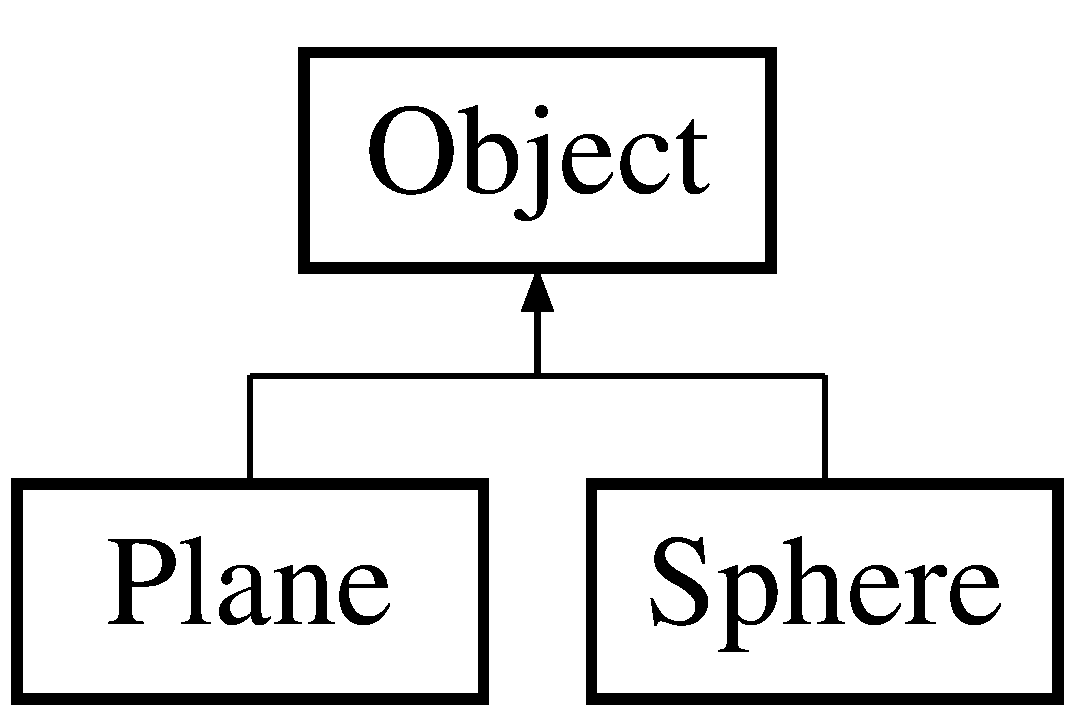
\includegraphics[height=2.000000cm]{class_object}
\end{center}
\end{figure}
\subsection*{Public Member Functions}
\begin{DoxyCompactItemize}
\item 
virtual glm\+::dvec3 \mbox{\hyperlink{class_object_a71cb3da0e19b83f2558bf406abc9db68}{get\+Postion}} ()=0
\item 
virtual \mbox{\hyperlink{struct_intersect}{Intersect}} \mbox{\hyperlink{class_object_a16d022cf54624baea89c542a44e6db26}{intersect}} (const \mbox{\hyperlink{struct_ray}{Ray}} \&r, double bias)=0
\item 
virtual void \mbox{\hyperlink{class_object_ad81452e5a38455eff025d85ef1da7307}{print}} ()=0
\item 
virtual glm\+::dvec3 \mbox{\hyperlink{class_object_a96a5bb5dcad4c340caa1d806fb5bd572}{get\+Colour}} ()=0
\item 
virtual glm\+::dvec3 \mbox{\hyperlink{class_object_abecc5668197c7222b5c9180a9738f69b}{get\+Colour}} (const \mbox{\hyperlink{class_light}{Light}} \&light, const \mbox{\hyperlink{struct_intersect}{Intersect}} \&hit, const glm\+::dvec3 \&cam\+Pos)=0
\end{DoxyCompactItemize}


\subsection{Detailed Description}
A pure virtual parent class for any physical object in this scene. 

Definition at line 16 of file object.\+h.



\subsection{Member Function Documentation}
\mbox{\Hypertarget{class_object_a96a5bb5dcad4c340caa1d806fb5bd572}\label{class_object_a96a5bb5dcad4c340caa1d806fb5bd572}} 
\index{Object@{Object}!get\+Colour@{get\+Colour}}
\index{get\+Colour@{get\+Colour}!Object@{Object}}
\subsubsection{\texorpdfstring{get\+Colour()}{getColour()}\hspace{0.1cm}{\footnotesize\ttfamily [1/2]}}
{\footnotesize\ttfamily virtual glm\+::dvec3 Object\+::get\+Colour (\begin{DoxyParamCaption}{ }\end{DoxyParamCaption})\hspace{0.3cm}{\ttfamily [pure virtual]}}



Implemented in \mbox{\hyperlink{class_sphere_a700025702852f2f6c888c7dbd720ea76}{Sphere}}, and \mbox{\hyperlink{class_plane_acd86caefd4ff1bf35f2719b1bef6afd8}{Plane}}.

\mbox{\Hypertarget{class_object_abecc5668197c7222b5c9180a9738f69b}\label{class_object_abecc5668197c7222b5c9180a9738f69b}} 
\index{Object@{Object}!get\+Colour@{get\+Colour}}
\index{get\+Colour@{get\+Colour}!Object@{Object}}
\subsubsection{\texorpdfstring{get\+Colour()}{getColour()}\hspace{0.1cm}{\footnotesize\ttfamily [2/2]}}
{\footnotesize\ttfamily virtual glm\+::dvec3 Object\+::get\+Colour (\begin{DoxyParamCaption}\item[{const \mbox{\hyperlink{class_light}{Light}} \&}]{light,  }\item[{const \mbox{\hyperlink{struct_intersect}{Intersect}} \&}]{hit,  }\item[{const glm\+::dvec3 \&}]{cam\+Pos }\end{DoxyParamCaption})\hspace{0.3cm}{\ttfamily [pure virtual]}}



Implemented in \mbox{\hyperlink{class_sphere_ac5c6bbcd43b8caabe4a23ba3e53d414a}{Sphere}}, and \mbox{\hyperlink{class_plane_a05e58028f795833a1ee68b374597fa3a}{Plane}}.

\mbox{\Hypertarget{class_object_a71cb3da0e19b83f2558bf406abc9db68}\label{class_object_a71cb3da0e19b83f2558bf406abc9db68}} 
\index{Object@{Object}!get\+Postion@{get\+Postion}}
\index{get\+Postion@{get\+Postion}!Object@{Object}}
\subsubsection{\texorpdfstring{get\+Postion()}{getPostion()}}
{\footnotesize\ttfamily virtual glm\+::dvec3 Object\+::get\+Postion (\begin{DoxyParamCaption}{ }\end{DoxyParamCaption})\hspace{0.3cm}{\ttfamily [pure virtual]}}



Implemented in \mbox{\hyperlink{class_sphere_abcc01a6057eb30df9605ce3786b6c47c}{Sphere}}, and \mbox{\hyperlink{class_plane_ab49db9185e5489809dc13135a5231109}{Plane}}.

\mbox{\Hypertarget{class_object_a16d022cf54624baea89c542a44e6db26}\label{class_object_a16d022cf54624baea89c542a44e6db26}} 
\index{Object@{Object}!intersect@{intersect}}
\index{intersect@{intersect}!Object@{Object}}
\subsubsection{\texorpdfstring{intersect()}{intersect()}}
{\footnotesize\ttfamily virtual \mbox{\hyperlink{struct_intersect}{Intersect}} Object\+::intersect (\begin{DoxyParamCaption}\item[{const \mbox{\hyperlink{struct_ray}{Ray}} \&}]{r,  }\item[{double}]{bias }\end{DoxyParamCaption})\hspace{0.3cm}{\ttfamily [pure virtual]}}



Implemented in \mbox{\hyperlink{class_sphere_a3ba8c2a4bc8108b244f35e71c14b952d}{Sphere}}, and \mbox{\hyperlink{class_plane_ab636b2a91165088ba60dac02aaf89785}{Plane}}.

\mbox{\Hypertarget{class_object_ad81452e5a38455eff025d85ef1da7307}\label{class_object_ad81452e5a38455eff025d85ef1da7307}} 
\index{Object@{Object}!print@{print}}
\index{print@{print}!Object@{Object}}
\subsubsection{\texorpdfstring{print()}{print()}}
{\footnotesize\ttfamily virtual void Object\+::print (\begin{DoxyParamCaption}{ }\end{DoxyParamCaption})\hspace{0.3cm}{\ttfamily [pure virtual]}}



Implemented in \mbox{\hyperlink{class_sphere_a95537121c5308b7b250f4a53171303ef}{Sphere}}, and \mbox{\hyperlink{class_plane_a3d9139793b931279e3dcd1fd80a263c7}{Plane}}.



The documentation for this class was generated from the following file\+:\begin{DoxyCompactItemize}
\item 
\mbox{\hyperlink{object_8h}{object.\+h}}\end{DoxyCompactItemize}

\hypertarget{class_plane}{}\section{Plane Class Reference}
\label{class_plane}\index{Plane@{Plane}}


Child of \mbox{\hyperlink{class_object}{Object}}. This class represents infinte planes that can be placed in the scene.  




{\ttfamily \#include $<$plane.\+h$>$}

Inheritance diagram for Plane\+:\begin{figure}[H]
\begin{center}
\leavevmode
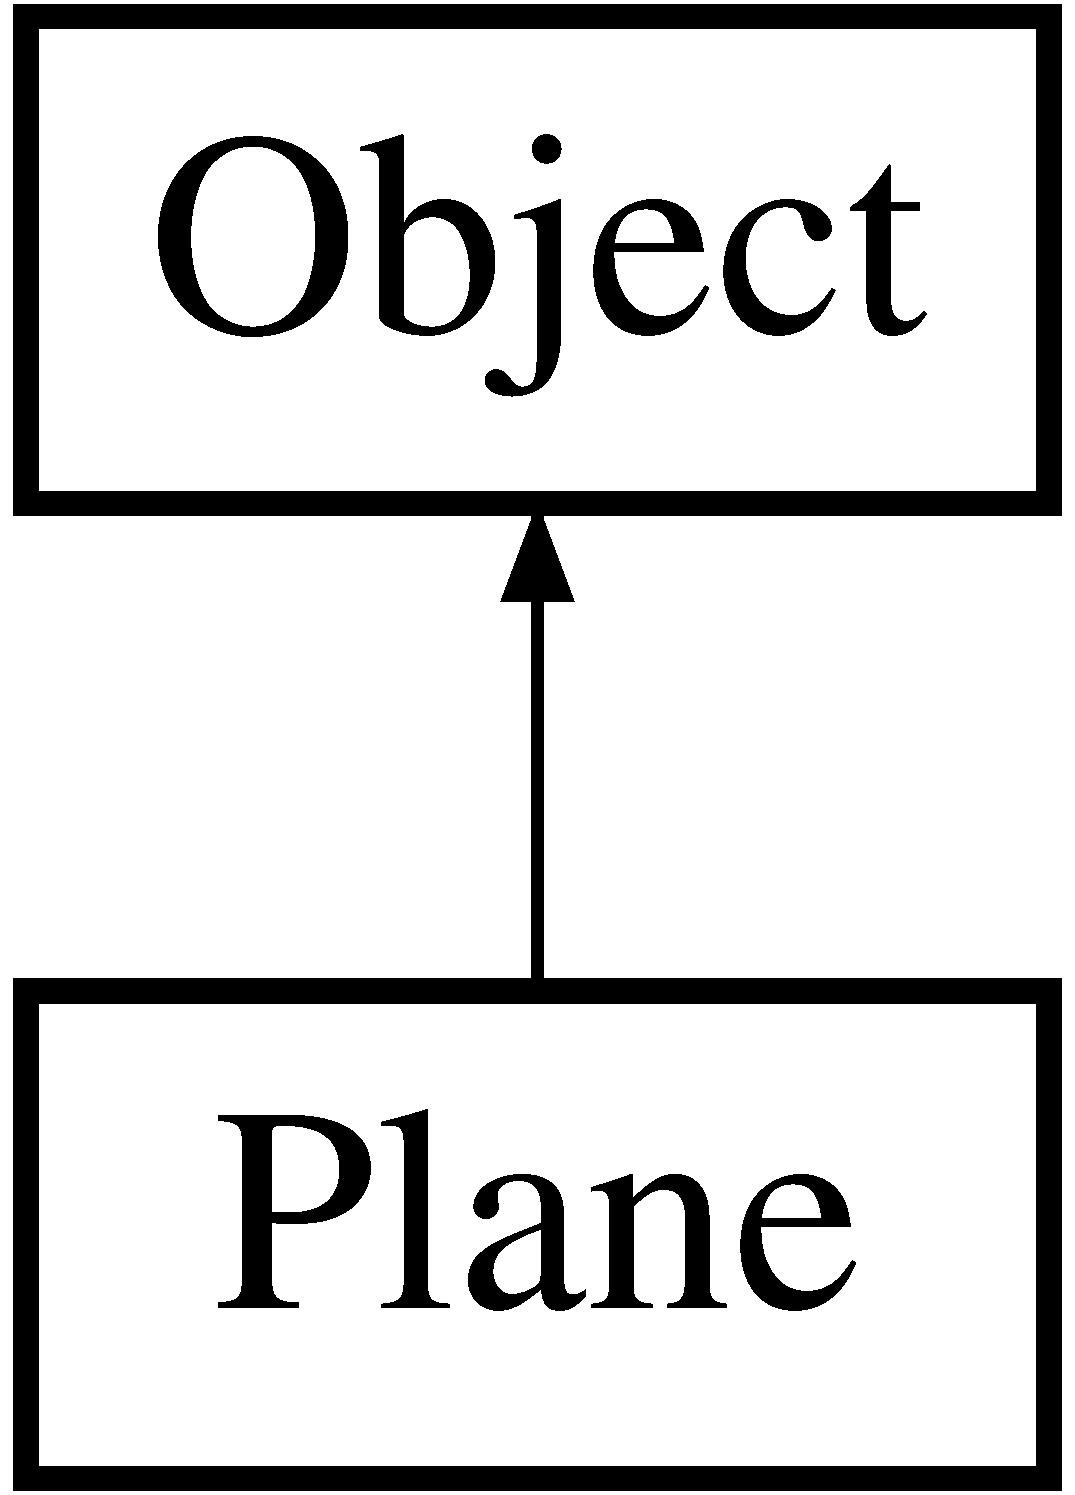
\includegraphics[height=2.000000cm]{class_plane}
\end{center}
\end{figure}
\subsection*{Public Member Functions}
\begin{DoxyCompactItemize}
\item 
\mbox{\hyperlink{class_plane_aeb002db84ff90de81df472544c35dbca}{Plane}} (glm\+::dvec3 norm, glm\+::dvec3 pos, glm\+::dvec3 amb, glm\+::dvec3 dif, glm\+::dvec3 spe, double shine)
\begin{DoxyCompactList}\small\item\em Just the basic constructor. \end{DoxyCompactList}\item 
glm\+::dvec3 \mbox{\hyperlink{class_plane_ab49db9185e5489809dc13135a5231109}{get\+Postion}} () override
\item 
\mbox{\hyperlink{struct_intersect}{Intersect}} \mbox{\hyperlink{class_plane_ab636b2a91165088ba60dac02aaf89785}{intersect}} (const \mbox{\hyperlink{struct_ray}{Ray}} \&r, double bias) override
\begin{DoxyCompactList}\small\item\em Returns the position of the plane. \end{DoxyCompactList}\item 
void \mbox{\hyperlink{class_plane_a3d9139793b931279e3dcd1fd80a263c7}{print}} () override
\begin{DoxyCompactList}\small\item\em Prints a nicely formatted string with all the plane\textquotesingle{}s stats. \end{DoxyCompactList}\item 
glm\+::dvec3 \mbox{\hyperlink{class_plane_acd86caefd4ff1bf35f2719b1bef6afd8}{get\+Colour}} () override
\begin{DoxyCompactList}\small\item\em Returns the ambient colour. \end{DoxyCompactList}\item 
glm\+::dvec3 \mbox{\hyperlink{class_plane_a05e58028f795833a1ee68b374597fa3a}{get\+Colour}} (const \mbox{\hyperlink{class_light}{Light}} \&light, const \mbox{\hyperlink{struct_intersect}{Intersect}} \&hit, const glm\+::dvec3 \&cam\+Pos) override
\begin{DoxyCompactList}\small\item\em Runs \mbox{\hyperlink{util_8h_add552e26ff1418c78cbcb09b18ab0f44}{calculate\+\_\+colour}} and returns the result. \end{DoxyCompactList}\end{DoxyCompactItemize}


\subsection{Detailed Description}
Child of \mbox{\hyperlink{class_object}{Object}}. This class represents infinte planes that can be placed in the scene. 

Definition at line 15 of file plane.\+h.



\subsection{Constructor \& Destructor Documentation}
\mbox{\Hypertarget{class_plane_aeb002db84ff90de81df472544c35dbca}\label{class_plane_aeb002db84ff90de81df472544c35dbca}} 
\index{Plane@{Plane}!Plane@{Plane}}
\index{Plane@{Plane}!Plane@{Plane}}
\subsubsection{\texorpdfstring{Plane()}{Plane()}}
{\footnotesize\ttfamily Plane\+::\+Plane (\begin{DoxyParamCaption}\item[{glm\+::dvec3}]{norm,  }\item[{glm\+::dvec3}]{pos,  }\item[{glm\+::dvec3}]{amb,  }\item[{glm\+::dvec3}]{dif,  }\item[{glm\+::dvec3}]{spe,  }\item[{double}]{shine }\end{DoxyParamCaption})}



Just the basic constructor. 



Definition at line 3 of file plane.\+cpp.



\subsection{Member Function Documentation}
\mbox{\Hypertarget{class_plane_acd86caefd4ff1bf35f2719b1bef6afd8}\label{class_plane_acd86caefd4ff1bf35f2719b1bef6afd8}} 
\index{Plane@{Plane}!get\+Colour@{get\+Colour}}
\index{get\+Colour@{get\+Colour}!Plane@{Plane}}
\subsubsection{\texorpdfstring{get\+Colour()}{getColour()}\hspace{0.1cm}{\footnotesize\ttfamily [1/2]}}
{\footnotesize\ttfamily glm\+::dvec3 Plane\+::get\+Colour (\begin{DoxyParamCaption}{ }\end{DoxyParamCaption})\hspace{0.3cm}{\ttfamily [override]}, {\ttfamily [virtual]}}



Returns the ambient colour. 



Implements \mbox{\hyperlink{class_object_a96a5bb5dcad4c340caa1d806fb5bd572}{Object}}.



Definition at line 56 of file plane.\+cpp.

\mbox{\Hypertarget{class_plane_a05e58028f795833a1ee68b374597fa3a}\label{class_plane_a05e58028f795833a1ee68b374597fa3a}} 
\index{Plane@{Plane}!get\+Colour@{get\+Colour}}
\index{get\+Colour@{get\+Colour}!Plane@{Plane}}
\subsubsection{\texorpdfstring{get\+Colour()}{getColour()}\hspace{0.1cm}{\footnotesize\ttfamily [2/2]}}
{\footnotesize\ttfamily glm\+::dvec3 Plane\+::get\+Colour (\begin{DoxyParamCaption}\item[{const \mbox{\hyperlink{class_light}{Light}} \&}]{light,  }\item[{const \mbox{\hyperlink{struct_intersect}{Intersect}} \&}]{hit,  }\item[{const glm\+::dvec3 \&}]{cam\+Pos }\end{DoxyParamCaption})\hspace{0.3cm}{\ttfamily [override]}, {\ttfamily [virtual]}}



Runs \mbox{\hyperlink{util_8h_add552e26ff1418c78cbcb09b18ab0f44}{calculate\+\_\+colour}} and returns the result. 



Implements \mbox{\hyperlink{class_object_abecc5668197c7222b5c9180a9738f69b}{Object}}.



Definition at line 61 of file plane.\+cpp.

\mbox{\Hypertarget{class_plane_ab49db9185e5489809dc13135a5231109}\label{class_plane_ab49db9185e5489809dc13135a5231109}} 
\index{Plane@{Plane}!get\+Postion@{get\+Postion}}
\index{get\+Postion@{get\+Postion}!Plane@{Plane}}
\subsubsection{\texorpdfstring{get\+Postion()}{getPostion()}}
{\footnotesize\ttfamily glm\+::dvec3 Plane\+::get\+Postion (\begin{DoxyParamCaption}{ }\end{DoxyParamCaption})\hspace{0.3cm}{\ttfamily [inline]}, {\ttfamily [override]}, {\ttfamily [virtual]}}



Implements \mbox{\hyperlink{class_object_a71cb3da0e19b83f2558bf406abc9db68}{Object}}.



Definition at line 24 of file plane.\+h.

\mbox{\Hypertarget{class_plane_ab636b2a91165088ba60dac02aaf89785}\label{class_plane_ab636b2a91165088ba60dac02aaf89785}} 
\index{Plane@{Plane}!intersect@{intersect}}
\index{intersect@{intersect}!Plane@{Plane}}
\subsubsection{\texorpdfstring{intersect()}{intersect()}}
{\footnotesize\ttfamily \mbox{\hyperlink{struct_intersect}{Intersect}} Plane\+::intersect (\begin{DoxyParamCaption}\item[{const \mbox{\hyperlink{struct_ray}{Ray}} \&}]{r,  }\item[{double}]{bias }\end{DoxyParamCaption})\hspace{0.3cm}{\ttfamily [override]}, {\ttfamily [virtual]}}



Returns the position of the plane. 

Checks if a ray intersects with the plane. Returns an \mbox{\hyperlink{struct_intersect}{Intersect}} with contact true or false. 

Implements \mbox{\hyperlink{class_object_a16d022cf54624baea89c542a44e6db26}{Object}}.



Definition at line 12 of file plane.\+cpp.

\mbox{\Hypertarget{class_plane_a3d9139793b931279e3dcd1fd80a263c7}\label{class_plane_a3d9139793b931279e3dcd1fd80a263c7}} 
\index{Plane@{Plane}!print@{print}}
\index{print@{print}!Plane@{Plane}}
\subsubsection{\texorpdfstring{print()}{print()}}
{\footnotesize\ttfamily void Plane\+::print (\begin{DoxyParamCaption}{ }\end{DoxyParamCaption})\hspace{0.3cm}{\ttfamily [override]}, {\ttfamily [virtual]}}



Prints a nicely formatted string with all the plane\textquotesingle{}s stats. 



Implements \mbox{\hyperlink{class_object_ad81452e5a38455eff025d85ef1da7307}{Object}}.



Definition at line 46 of file plane.\+cpp.



The documentation for this class was generated from the following files\+:\begin{DoxyCompactItemize}
\item 
\mbox{\hyperlink{plane_8h}{plane.\+h}}\item 
\mbox{\hyperlink{plane_8cpp}{plane.\+cpp}}\end{DoxyCompactItemize}

\hypertarget{struct_ray}{}\section{Ray Struct Reference}
\label{struct_ray}\index{Ray@{Ray}}


A \mbox{\hyperlink{struct_ray}{Ray}} that can be fired from things.  




{\ttfamily \#include $<$structs.\+h$>$}

\subsection*{Public Attributes}
\begin{DoxyCompactItemize}
\item 
glm\+::dvec3 \mbox{\hyperlink{struct_ray_a78a1cbfb1bd302b4c1790fbe41845d31}{org}}
\begin{DoxyCompactList}\small\item\em The origin of the ray. \mbox{\hyperlink{struct_ray_a78a1cbfb1bd302b4c1790fbe41845d31}{org}}. \end{DoxyCompactList}\item 
glm\+::dvec3 \mbox{\hyperlink{struct_ray_a80a47e5925e6f8d150e6ade067590520}{dir}}
\begin{DoxyCompactList}\small\item\em The direction of the ray. Make sure to normalize!!! \mbox{\hyperlink{struct_ray_a80a47e5925e6f8d150e6ade067590520}{dir}}. \end{DoxyCompactList}\end{DoxyCompactItemize}


\subsection{Detailed Description}
A \mbox{\hyperlink{struct_ray}{Ray}} that can be fired from things. 

Definition at line 14 of file structs.\+h.



\subsection{Member Data Documentation}
\mbox{\Hypertarget{struct_ray_a80a47e5925e6f8d150e6ade067590520}\label{struct_ray_a80a47e5925e6f8d150e6ade067590520}} 
\index{Ray@{Ray}!dir@{dir}}
\index{dir@{dir}!Ray@{Ray}}
\subsubsection{\texorpdfstring{dir}{dir}}
{\footnotesize\ttfamily glm\+::dvec3 Ray\+::dir}



The direction of the ray. Make sure to normalize!!! \mbox{\hyperlink{struct_ray_a80a47e5925e6f8d150e6ade067590520}{dir}}. 



Definition at line 16 of file structs.\+h.

\mbox{\Hypertarget{struct_ray_a78a1cbfb1bd302b4c1790fbe41845d31}\label{struct_ray_a78a1cbfb1bd302b4c1790fbe41845d31}} 
\index{Ray@{Ray}!org@{org}}
\index{org@{org}!Ray@{Ray}}
\subsubsection{\texorpdfstring{org}{org}}
{\footnotesize\ttfamily glm\+::dvec3 Ray\+::org}



The origin of the ray. \mbox{\hyperlink{struct_ray_a78a1cbfb1bd302b4c1790fbe41845d31}{org}}. 



Definition at line 15 of file structs.\+h.



The documentation for this struct was generated from the following file\+:\begin{DoxyCompactItemize}
\item 
\mbox{\hyperlink{structs_8h}{structs.\+h}}\end{DoxyCompactItemize}

\hypertarget{class_sphere}{}\section{Sphere Class Reference}
\label{class_sphere}\index{Sphere@{Sphere}}


Child of \mbox{\hyperlink{class_object}{Object}}. This class represents Spheres that can be placed in the scene.  




{\ttfamily \#include $<$sphere.\+h$>$}

Inheritance diagram for Sphere\+:\begin{figure}[H]
\begin{center}
\leavevmode
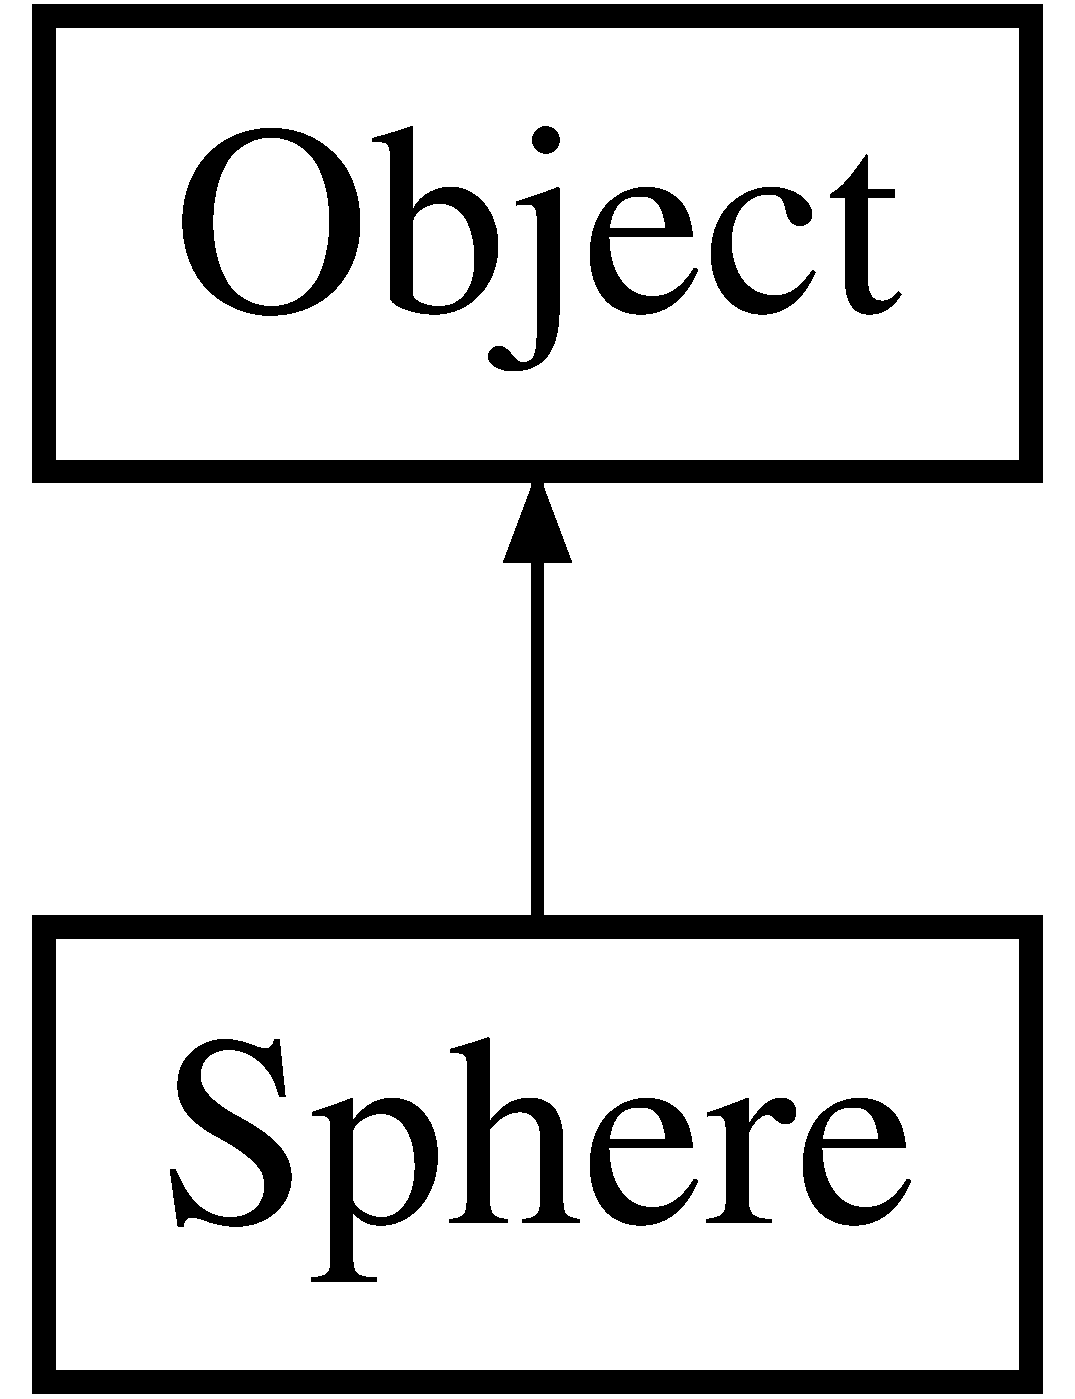
\includegraphics[height=2.000000cm]{class_sphere}
\end{center}
\end{figure}
\subsection*{Public Member Functions}
\begin{DoxyCompactItemize}
\item 
\mbox{\hyperlink{class_sphere_ac5331c3b7a05c78676a39ea7d30791ca}{Sphere}} (glm\+::vec3 pos, int rad, glm\+::vec3 amb, glm\+::vec3 dif, glm\+::vec3 spe, float shi)
\begin{DoxyCompactList}\small\item\em Just the basic constructor. \end{DoxyCompactList}\item 
glm\+::vec3 \mbox{\hyperlink{class_sphere_a6e2f290f9632e8da3d8dd90dc74997ac}{get\+Postion}} () override
\item 
\mbox{\hyperlink{struct_intersect}{Intersect}} \mbox{\hyperlink{class_sphere_a8d2ea6e36b5c23330e08861bb723e2a4}{intersect}} (const \mbox{\hyperlink{struct_ray}{Ray}} \&r) override
\begin{DoxyCompactList}\small\item\em Returns the position of the sphere\textquotesingle{}s centre. \end{DoxyCompactList}\item 
void \mbox{\hyperlink{class_sphere_a95537121c5308b7b250f4a53171303ef}{print}} () override
\begin{DoxyCompactList}\small\item\em Prints a nicely formatted string with all the sphere\textquotesingle{}s stats. \end{DoxyCompactList}\item 
glm\+::vec3 \mbox{\hyperlink{class_sphere_abc6455e04b563fb57b91f12183fa4d18}{get\+Colour}} () override
\begin{DoxyCompactList}\small\item\em Returns the ambient colour. \end{DoxyCompactList}\item 
glm\+::vec3 \mbox{\hyperlink{class_sphere_a0ce51c06baaea1c35129b17b5132ff58}{get\+Colour}} (const \mbox{\hyperlink{class_light}{Light}} \&light, const \mbox{\hyperlink{struct_intersect}{Intersect}} \&hit, const glm\+::vec3 \&cam\+Pos) override
\begin{DoxyCompactList}\small\item\em Calculates the norm for the point of contact then runs \mbox{\hyperlink{util_8h_ae9aaa22b1b1c0249f8617f45eb99ad55}{calculate\+\_\+colour}}. \end{DoxyCompactList}\end{DoxyCompactItemize}


\subsection{Detailed Description}
Child of \mbox{\hyperlink{class_object}{Object}}. This class represents Spheres that can be placed in the scene. 

Definition at line 16 of file sphere.\+h.



\subsection{Constructor \& Destructor Documentation}
\mbox{\Hypertarget{class_sphere_ac5331c3b7a05c78676a39ea7d30791ca}\label{class_sphere_ac5331c3b7a05c78676a39ea7d30791ca}} 
\index{Sphere@{Sphere}!Sphere@{Sphere}}
\index{Sphere@{Sphere}!Sphere@{Sphere}}
\subsubsection{\texorpdfstring{Sphere()}{Sphere()}}
{\footnotesize\ttfamily Sphere\+::\+Sphere (\begin{DoxyParamCaption}\item[{glm\+::vec3}]{pos,  }\item[{int}]{rad,  }\item[{glm\+::vec3}]{amb,  }\item[{glm\+::vec3}]{dif,  }\item[{glm\+::vec3}]{spe,  }\item[{float}]{shi }\end{DoxyParamCaption})}



Just the basic constructor. 



Definition at line 3 of file sphere.\+cpp.



\subsection{Member Function Documentation}
\mbox{\Hypertarget{class_sphere_abc6455e04b563fb57b91f12183fa4d18}\label{class_sphere_abc6455e04b563fb57b91f12183fa4d18}} 
\index{Sphere@{Sphere}!get\+Colour@{get\+Colour}}
\index{get\+Colour@{get\+Colour}!Sphere@{Sphere}}
\subsubsection{\texorpdfstring{get\+Colour()}{getColour()}\hspace{0.1cm}{\footnotesize\ttfamily [1/2]}}
{\footnotesize\ttfamily glm\+::vec3 Sphere\+::get\+Colour (\begin{DoxyParamCaption}{ }\end{DoxyParamCaption})\hspace{0.3cm}{\ttfamily [override]}, {\ttfamily [virtual]}}



Returns the ambient colour. 



Implements \mbox{\hyperlink{class_object_a0a966fb37be861cbaacb834ef7b89d8a}{Object}}.



Definition at line 66 of file sphere.\+cpp.

\mbox{\Hypertarget{class_sphere_a0ce51c06baaea1c35129b17b5132ff58}\label{class_sphere_a0ce51c06baaea1c35129b17b5132ff58}} 
\index{Sphere@{Sphere}!get\+Colour@{get\+Colour}}
\index{get\+Colour@{get\+Colour}!Sphere@{Sphere}}
\subsubsection{\texorpdfstring{get\+Colour()}{getColour()}\hspace{0.1cm}{\footnotesize\ttfamily [2/2]}}
{\footnotesize\ttfamily glm\+::vec3 Sphere\+::get\+Colour (\begin{DoxyParamCaption}\item[{const \mbox{\hyperlink{class_light}{Light}} \&}]{light,  }\item[{const \mbox{\hyperlink{struct_intersect}{Intersect}} \&}]{hit,  }\item[{const glm\+::vec3 \&}]{cam\+Pos }\end{DoxyParamCaption})\hspace{0.3cm}{\ttfamily [override]}, {\ttfamily [virtual]}}



Calculates the norm for the point of contact then runs \mbox{\hyperlink{util_8h_ae9aaa22b1b1c0249f8617f45eb99ad55}{calculate\+\_\+colour}}. 



Implements \mbox{\hyperlink{class_object_aac162b545913d7aeab851204d3f04ebf}{Object}}.



Definition at line 71 of file sphere.\+cpp.

\mbox{\Hypertarget{class_sphere_a6e2f290f9632e8da3d8dd90dc74997ac}\label{class_sphere_a6e2f290f9632e8da3d8dd90dc74997ac}} 
\index{Sphere@{Sphere}!get\+Postion@{get\+Postion}}
\index{get\+Postion@{get\+Postion}!Sphere@{Sphere}}
\subsubsection{\texorpdfstring{get\+Postion()}{getPostion()}}
{\footnotesize\ttfamily glm\+::vec3 Sphere\+::get\+Postion (\begin{DoxyParamCaption}{ }\end{DoxyParamCaption})\hspace{0.3cm}{\ttfamily [inline]}, {\ttfamily [override]}, {\ttfamily [virtual]}}



Implements \mbox{\hyperlink{class_object_ac29e04a255155b791d69b97820423efa}{Object}}.



Definition at line 25 of file sphere.\+h.

\mbox{\Hypertarget{class_sphere_a8d2ea6e36b5c23330e08861bb723e2a4}\label{class_sphere_a8d2ea6e36b5c23330e08861bb723e2a4}} 
\index{Sphere@{Sphere}!intersect@{intersect}}
\index{intersect@{intersect}!Sphere@{Sphere}}
\subsubsection{\texorpdfstring{intersect()}{intersect()}}
{\footnotesize\ttfamily \mbox{\hyperlink{struct_intersect}{Intersect}} Sphere\+::intersect (\begin{DoxyParamCaption}\item[{const \mbox{\hyperlink{struct_ray}{Ray}} \&}]{r }\end{DoxyParamCaption})\hspace{0.3cm}{\ttfamily [override]}, {\ttfamily [virtual]}}



Returns the position of the sphere\textquotesingle{}s centre. 

Checks if a ray intersects with the sphere. Returns an \mbox{\hyperlink{struct_intersect}{Intersect}} with contact true or false. 

Implements \mbox{\hyperlink{class_object_a27b26f69f1fcb4dc72eca40ac0d20ea6}{Object}}.



Definition at line 12 of file sphere.\+cpp.

\mbox{\Hypertarget{class_sphere_a95537121c5308b7b250f4a53171303ef}\label{class_sphere_a95537121c5308b7b250f4a53171303ef}} 
\index{Sphere@{Sphere}!print@{print}}
\index{print@{print}!Sphere@{Sphere}}
\subsubsection{\texorpdfstring{print()}{print()}}
{\footnotesize\ttfamily void Sphere\+::print (\begin{DoxyParamCaption}{ }\end{DoxyParamCaption})\hspace{0.3cm}{\ttfamily [override]}, {\ttfamily [virtual]}}



Prints a nicely formatted string with all the sphere\textquotesingle{}s stats. 



Implements \mbox{\hyperlink{class_object_ad81452e5a38455eff025d85ef1da7307}{Object}}.



Definition at line 56 of file sphere.\+cpp.



The documentation for this class was generated from the following files\+:\begin{DoxyCompactItemize}
\item 
\mbox{\hyperlink{sphere_8h}{sphere.\+h}}\item 
\mbox{\hyperlink{sphere_8cpp}{sphere.\+cpp}}\end{DoxyCompactItemize}

\chapter{File Documentation}
\hypertarget{camera_8cpp}{}\section{camera.\+cpp File Reference}
\label{camera_8cpp}\index{camera.\+cpp@{camera.\+cpp}}
{\ttfamily \#include \char`\"{}camera.\+h\char`\"{}}\newline

\hypertarget{camera_8h}{}\section{camera.\+h File Reference}
\label{camera_8h}\index{camera.\+h@{camera.\+h}}


The header for the camera class.  


{\ttfamily \#include \char`\"{}libs.\+h\char`\"{}}\newline
\subsection*{Classes}
\begin{DoxyCompactItemize}
\item 
class \mbox{\hyperlink{class_camera}{Camera}}
\end{DoxyCompactItemize}


\subsection{Detailed Description}
The header for the camera class. 

\begin{DoxyAuthor}{Author}
Mottel Zirkind 
\end{DoxyAuthor}

\hypertarget{libs_8h}{}\section{libs.\+h File Reference}
\label{libs_8h}\index{libs.\+h@{libs.\+h}}


The header for external libraries that are used everywhere. Also defines T\+\_\+\+B\+I\+AS which helps with acne.  


{\ttfamily \#include $<$iostream$>$}\newline
{\ttfamily \#include $<$iomanip$>$}\newline
{\ttfamily \#include $<$ctime$>$}\newline
{\ttfamily \#include $<$string$>$}\newline
{\ttfamily \#include $<$sstream$>$}\newline
{\ttfamily \#include $<$fstream$>$}\newline
{\ttfamily \#include $<$vector$>$}\newline
{\ttfamily \#include $<$glm/glm.\+hpp$>$}\newline
{\ttfamily \#include $<$glm/ext.\+hpp$>$}\newline
{\ttfamily \#include $<$glm/gtc/epsilon.\+hpp$>$}\newline
{\ttfamily \#include $<$C\+Img.\+h$>$}\newline
\subsection*{Macros}
\begin{DoxyCompactItemize}
\item 
\mbox{\Hypertarget{libs_8h_aa271a028eb2491a0227d7b5cee409a78}\label{libs_8h_aa271a028eb2491a0227d7b5cee409a78}} 
\#define {\bfseries cimg\+\_\+use\+\_\+png}
\item 
\mbox{\Hypertarget{libs_8h_a38549847157001dda452b392cbf87ed6}\label{libs_8h_a38549847157001dda452b392cbf87ed6}} 
\#define {\bfseries cimg\+\_\+use\+\_\+jpeg}
\item 
\mbox{\Hypertarget{libs_8h_a7b2bbc905e99be30eb5b7860b88b252d}\label{libs_8h_a7b2bbc905e99be30eb5b7860b88b252d}} 
\#define {\bfseries T\+\_\+\+B\+I\+AS}~0.\+025f
\end{DoxyCompactItemize}


\subsection{Detailed Description}
The header for external libraries that are used everywhere. Also defines T\+\_\+\+B\+I\+AS which helps with acne. 

\begin{DoxyAuthor}{Author}
Mottel Zirkind 
\end{DoxyAuthor}

\hypertarget{light_8cpp}{}\section{light.\+cpp File Reference}
\label{light_8cpp}\index{light.\+cpp@{light.\+cpp}}
{\ttfamily \#include \char`\"{}light.\+h\char`\"{}}\newline

\hypertarget{light_8h}{}\section{light.\+h File Reference}
\label{light_8h}\index{light.\+h@{light.\+h}}


The header for the light class.  


{\ttfamily \#include \char`\"{}libs.\+h\char`\"{}}\newline
{\ttfamily \#include \char`\"{}util.\+h\char`\"{}}\newline
{\ttfamily \#include \char`\"{}structs.\+h\char`\"{}}\newline
\subsection*{Classes}
\begin{DoxyCompactItemize}
\item 
class \mbox{\hyperlink{class_light}{Light}}
\begin{DoxyCompactList}\small\item\em \mbox{\hyperlink{class_light}{Light}} class could basically be a struct. This is a really minimal class that just store all the light\textquotesingle{}s data. \end{DoxyCompactList}\end{DoxyCompactItemize}


\subsection{Detailed Description}
The header for the light class. 

\begin{DoxyAuthor}{Author}
Mottel Zirkind 
\end{DoxyAuthor}

\hypertarget{main_8cpp}{}\section{main.\+cpp File Reference}
\label{main_8cpp}\index{main.\+cpp@{main.\+cpp}}
{\ttfamily \#include \char`\"{}libs.\+h\char`\"{}}\newline
{\ttfamily \#include \char`\"{}util.\+h\char`\"{}}\newline
{\ttfamily \#include \char`\"{}sceneload.\+h\char`\"{}}\newline
\subsection*{Macros}
\begin{DoxyCompactItemize}
\item 
\#define \mbox{\hyperlink{main_8cpp_a0fae658d4f8fc42f49d50a01db3c93a2}{show\+\_\+pic}}~false
\item 
\#define \mbox{\hyperlink{main_8cpp_a985821aa28574e23e520bfde1a694921}{mot\+\_\+log}}~false
\end{DoxyCompactItemize}
\subsection*{Functions}
\begin{DoxyCompactItemize}
\item 
int \mbox{\hyperlink{main_8cpp_ac0f2228420376f4db7e1274f2b41667c}{main}} (int argc, const char $\ast$argv\mbox{[}$\,$\mbox{]})
\end{DoxyCompactItemize}
\subsection*{Variables}
\begin{DoxyCompactItemize}
\item 
std\+::string \mbox{\hyperlink{main_8cpp_a45ddb9af9deebcd9f0b060abff92da07}{scene}} = \char`\"{}scenes/scene1.\+txt\char`\"{}
\item 
double \mbox{\hyperlink{main_8cpp_a3e16e5822a9cea9b4940f8d5b93a358d}{ray\+\_\+bias}} = 0.\+00
\item 
double \mbox{\hyperlink{main_8cpp_a5907e790af6150a0dd0df4d0b5255503}{shadow\+\_\+bias}} = 0.\+0085
\end{DoxyCompactItemize}


\subsection{Macro Definition Documentation}
\mbox{\Hypertarget{main_8cpp_a985821aa28574e23e520bfde1a694921}\label{main_8cpp_a985821aa28574e23e520bfde1a694921}} 
\index{main.\+cpp@{main.\+cpp}!mot\+\_\+log@{mot\+\_\+log}}
\index{mot\+\_\+log@{mot\+\_\+log}!main.\+cpp@{main.\+cpp}}
\subsubsection{\texorpdfstring{mot\+\_\+log}{mot\_log}}
{\footnotesize\ttfamily \#define mot\+\_\+log~false}



Definition at line 2 of file main.\+cpp.

\mbox{\Hypertarget{main_8cpp_a0fae658d4f8fc42f49d50a01db3c93a2}\label{main_8cpp_a0fae658d4f8fc42f49d50a01db3c93a2}} 
\index{main.\+cpp@{main.\+cpp}!show\+\_\+pic@{show\+\_\+pic}}
\index{show\+\_\+pic@{show\+\_\+pic}!main.\+cpp@{main.\+cpp}}
\subsubsection{\texorpdfstring{show\+\_\+pic}{show\_pic}}
{\footnotesize\ttfamily \#define show\+\_\+pic~false}



Definition at line 1 of file main.\+cpp.



\subsection{Function Documentation}
\mbox{\Hypertarget{main_8cpp_ac0f2228420376f4db7e1274f2b41667c}\label{main_8cpp_ac0f2228420376f4db7e1274f2b41667c}} 
\index{main.\+cpp@{main.\+cpp}!main@{main}}
\index{main@{main}!main.\+cpp@{main.\+cpp}}
\subsubsection{\texorpdfstring{main()}{main()}}
{\footnotesize\ttfamily int main (\begin{DoxyParamCaption}\item[{int}]{argc,  }\item[{const char $\ast$}]{argv\mbox{[}$\,$\mbox{]} }\end{DoxyParamCaption})}



Definition at line 13 of file main.\+cpp.



\subsection{Variable Documentation}
\mbox{\Hypertarget{main_8cpp_a3e16e5822a9cea9b4940f8d5b93a358d}\label{main_8cpp_a3e16e5822a9cea9b4940f8d5b93a358d}} 
\index{main.\+cpp@{main.\+cpp}!ray\+\_\+bias@{ray\+\_\+bias}}
\index{ray\+\_\+bias@{ray\+\_\+bias}!main.\+cpp@{main.\+cpp}}
\subsubsection{\texorpdfstring{ray\+\_\+bias}{ray\_bias}}
{\footnotesize\ttfamily double ray\+\_\+bias = 0.\+00}



Definition at line 9 of file main.\+cpp.

\mbox{\Hypertarget{main_8cpp_a45ddb9af9deebcd9f0b060abff92da07}\label{main_8cpp_a45ddb9af9deebcd9f0b060abff92da07}} 
\index{main.\+cpp@{main.\+cpp}!scene@{scene}}
\index{scene@{scene}!main.\+cpp@{main.\+cpp}}
\subsubsection{\texorpdfstring{scene}{scene}}
{\footnotesize\ttfamily std\+::string scene = \char`\"{}scenes/scene1.\+txt\char`\"{}}



Definition at line 7 of file main.\+cpp.

\mbox{\Hypertarget{main_8cpp_a5907e790af6150a0dd0df4d0b5255503}\label{main_8cpp_a5907e790af6150a0dd0df4d0b5255503}} 
\index{main.\+cpp@{main.\+cpp}!shadow\+\_\+bias@{shadow\+\_\+bias}}
\index{shadow\+\_\+bias@{shadow\+\_\+bias}!main.\+cpp@{main.\+cpp}}
\subsubsection{\texorpdfstring{shadow\+\_\+bias}{shadow\_bias}}
{\footnotesize\ttfamily double shadow\+\_\+bias = 0.\+0085}



Definition at line 10 of file main.\+cpp.


\hypertarget{object_8h}{}\section{object.\+h File Reference}
\label{object_8h}\index{object.\+h@{object.\+h}}


The header for the object class.  


{\ttfamily \#include \char`\"{}libs.\+h\char`\"{}}\newline
{\ttfamily \#include \char`\"{}structs.\+h\char`\"{}}\newline
{\ttfamily \#include \char`\"{}light.\+h\char`\"{}}\newline
\subsection*{Classes}
\begin{DoxyCompactItemize}
\item 
class \mbox{\hyperlink{class_object}{Object}}
\begin{DoxyCompactList}\small\item\em A pure virtual parent class for any physical object in this scene. \end{DoxyCompactList}\end{DoxyCompactItemize}


\subsection{Detailed Description}
The header for the object class. 

\begin{DoxyAuthor}{Author}
Mottel Zirkind 
\end{DoxyAuthor}

\hypertarget{plane_8cpp}{}\section{plane.\+cpp File Reference}
\label{plane_8cpp}\index{plane.\+cpp@{plane.\+cpp}}
{\ttfamily \#include \char`\"{}plane.\+h\char`\"{}}\newline

\hypertarget{plane_8h}{}\section{plane.\+h File Reference}
\label{plane_8h}\index{plane.\+h@{plane.\+h}}


The header for the plane class.  


{\ttfamily \#include \char`\"{}object.\+h\char`\"{}}\newline
{\ttfamily \#include \char`\"{}structs.\+h\char`\"{}}\newline
{\ttfamily \#include \char`\"{}util.\+h\char`\"{}}\newline
\subsection*{Classes}
\begin{DoxyCompactItemize}
\item 
class \mbox{\hyperlink{class_plane}{Plane}}
\end{DoxyCompactItemize}


\subsection{Detailed Description}
The header for the plane class. 

\begin{DoxyAuthor}{Author}
Mottel Zirkind 
\end{DoxyAuthor}

\hypertarget{sceneload_8cpp}{}\section{sceneload.\+cpp File Reference}
\label{sceneload_8cpp}\index{sceneload.\+cpp@{sceneload.\+cpp}}
{\ttfamily \#include \char`\"{}sceneload.\+h\char`\"{}}\newline
\subsection*{Functions}
\begin{DoxyCompactItemize}
\item 
bool \mbox{\hyperlink{sceneload_8cpp_acc320c32cafcc507624d1678832581aa}{load\+\_\+scene}} (const std\+::string \&filepath)
\begin{DoxyCompactList}\small\item\em Loads the scene with a vec3 config and prints the read in results to terminal. Used for testing. \end{DoxyCompactList}\item 
bool \mbox{\hyperlink{sceneload_8cpp_a9aed10ae16077115b1d231d16ad5e47e}{load\+\_\+scene}} (const std\+::string \&filepath, std\+::vector$<$ \mbox{\hyperlink{class_object}{Object}} $\ast$$>$ \&things, std\+::vector$<$ \mbox{\hyperlink{class_light}{Light}} $\ast$$>$ \&lights, \mbox{\hyperlink{class_camera}{Camera}} $\ast$\&cam)
\begin{DoxyCompactList}\small\item\em Loads the scene with a vec3 config. \end{DoxyCompactList}\end{DoxyCompactItemize}


\subsection{Function Documentation}
\mbox{\Hypertarget{sceneload_8cpp_acc320c32cafcc507624d1678832581aa}\label{sceneload_8cpp_acc320c32cafcc507624d1678832581aa}} 
\index{sceneload.\+cpp@{sceneload.\+cpp}!load\+\_\+scene@{load\+\_\+scene}}
\index{load\+\_\+scene@{load\+\_\+scene}!sceneload.\+cpp@{sceneload.\+cpp}}
\subsubsection{\texorpdfstring{load\+\_\+scene()}{load\_scene()}\hspace{0.1cm}{\footnotesize\ttfamily [1/2]}}
{\footnotesize\ttfamily bool load\+\_\+scene (\begin{DoxyParamCaption}\item[{const std\+::string \&}]{filepath }\end{DoxyParamCaption})}



Loads the scene with a vec3 config and prints the read in results to terminal. Used for testing. 



Definition at line 5 of file sceneload.\+cpp.

\mbox{\Hypertarget{sceneload_8cpp_a9aed10ae16077115b1d231d16ad5e47e}\label{sceneload_8cpp_a9aed10ae16077115b1d231d16ad5e47e}} 
\index{sceneload.\+cpp@{sceneload.\+cpp}!load\+\_\+scene@{load\+\_\+scene}}
\index{load\+\_\+scene@{load\+\_\+scene}!sceneload.\+cpp@{sceneload.\+cpp}}
\subsubsection{\texorpdfstring{load\+\_\+scene()}{load\_scene()}\hspace{0.1cm}{\footnotesize\ttfamily [2/2]}}
{\footnotesize\ttfamily bool load\+\_\+scene (\begin{DoxyParamCaption}\item[{const std\+::string \&}]{filepath,  }\item[{std\+::vector$<$ \mbox{\hyperlink{class_object}{Object}} $\ast$$>$ \&}]{things,  }\item[{std\+::vector$<$ \mbox{\hyperlink{class_light}{Light}} $\ast$$>$ \&}]{lights,  }\item[{\mbox{\hyperlink{class_camera}{Camera}} $\ast$\&}]{cam }\end{DoxyParamCaption})}



Loads the scene with a vec3 config. 



Definition at line 155 of file sceneload.\+cpp.


\hypertarget{sceneload_8h}{}\section{sceneload.\+h File Reference}
\label{sceneload_8h}\index{sceneload.\+h@{sceneload.\+h}}


The scene loader. This version assumes a vec3 setup.  


{\ttfamily \#include \char`\"{}light.\+h\char`\"{}}\newline
{\ttfamily \#include \char`\"{}camera.\+h\char`\"{}}\newline
{\ttfamily \#include \char`\"{}sphere.\+h\char`\"{}}\newline
{\ttfamily \#include \char`\"{}plane.\+h\char`\"{}}\newline
\subsection*{Functions}
\begin{DoxyCompactItemize}
\item 
bool \mbox{\hyperlink{sceneload_8h_acc320c32cafcc507624d1678832581aa}{load\+\_\+scene}} (const std\+::string \&filepath)
\begin{DoxyCompactList}\small\item\em Loads the scene with a vec3 config and prints the read in results to terminal. Used for testing. \end{DoxyCompactList}\item 
bool \mbox{\hyperlink{sceneload_8h_a9aed10ae16077115b1d231d16ad5e47e}{load\+\_\+scene}} (const std\+::string \&filepath, std\+::vector$<$ \mbox{\hyperlink{class_object}{Object}} $\ast$$>$ \&things, std\+::vector$<$ \mbox{\hyperlink{class_light}{Light}} $\ast$$>$ \&lights, \mbox{\hyperlink{class_camera}{Camera}} $\ast$\&cam)
\begin{DoxyCompactList}\small\item\em Loads the scene with a vec3 config. \end{DoxyCompactList}\end{DoxyCompactItemize}


\subsection{Detailed Description}
The scene loader. This version assumes a vec3 setup. 

\begin{DoxyAuthor}{Author}
Mottel Zirkind 
\end{DoxyAuthor}


\subsection{Function Documentation}
\mbox{\Hypertarget{sceneload_8h_acc320c32cafcc507624d1678832581aa}\label{sceneload_8h_acc320c32cafcc507624d1678832581aa}} 
\index{sceneload.\+h@{sceneload.\+h}!load\+\_\+scene@{load\+\_\+scene}}
\index{load\+\_\+scene@{load\+\_\+scene}!sceneload.\+h@{sceneload.\+h}}
\subsubsection{\texorpdfstring{load\+\_\+scene()}{load\_scene()}\hspace{0.1cm}{\footnotesize\ttfamily [1/2]}}
{\footnotesize\ttfamily bool load\+\_\+scene (\begin{DoxyParamCaption}\item[{const std\+::string \&}]{filepath }\end{DoxyParamCaption})}



Loads the scene with a vec3 config and prints the read in results to terminal. Used for testing. 



Definition at line 5 of file sceneload.\+cpp.

\mbox{\Hypertarget{sceneload_8h_a9aed10ae16077115b1d231d16ad5e47e}\label{sceneload_8h_a9aed10ae16077115b1d231d16ad5e47e}} 
\index{sceneload.\+h@{sceneload.\+h}!load\+\_\+scene@{load\+\_\+scene}}
\index{load\+\_\+scene@{load\+\_\+scene}!sceneload.\+h@{sceneload.\+h}}
\subsubsection{\texorpdfstring{load\+\_\+scene()}{load\_scene()}\hspace{0.1cm}{\footnotesize\ttfamily [2/2]}}
{\footnotesize\ttfamily bool load\+\_\+scene (\begin{DoxyParamCaption}\item[{const std\+::string \&}]{filepath,  }\item[{std\+::vector$<$ \mbox{\hyperlink{class_object}{Object}} $\ast$$>$ \&}]{things,  }\item[{std\+::vector$<$ \mbox{\hyperlink{class_light}{Light}} $\ast$$>$ \&}]{lights,  }\item[{\mbox{\hyperlink{class_camera}{Camera}} $\ast$\&}]{cam }\end{DoxyParamCaption})}



Loads the scene with a vec3 config. 



Definition at line 155 of file sceneload.\+cpp.


\hypertarget{sphere_8cpp}{}\section{sphere.\+cpp File Reference}
\label{sphere_8cpp}\index{sphere.\+cpp@{sphere.\+cpp}}
{\ttfamily \#include \char`\"{}sphere.\+h\char`\"{}}\newline

\hypertarget{sphere_8h}{}\section{sphere.\+h File Reference}
\label{sphere_8h}\index{sphere.\+h@{sphere.\+h}}


The header for the sphere class.  


{\ttfamily \#include \char`\"{}object.\+h\char`\"{}}\newline
{\ttfamily \#include \char`\"{}util.\+h\char`\"{}}\newline
\subsection*{Classes}
\begin{DoxyCompactItemize}
\item 
class \mbox{\hyperlink{class_sphere}{Sphere}}
\end{DoxyCompactItemize}


\subsection{Detailed Description}
The header for the sphere class. 

\begin{DoxyAuthor}{Author}
Mottel Zirkind 
\end{DoxyAuthor}

\hypertarget{structs_8h}{}\section{structs.\+h File Reference}
\label{structs_8h}\index{structs.\+h@{structs.\+h}}


Home to the structs.  


{\ttfamily \#include \char`\"{}libs.\+h\char`\"{}}\newline
\subsection*{Classes}
\begin{DoxyCompactItemize}
\item 
struct \mbox{\hyperlink{struct_ray}{Ray}}
\begin{DoxyCompactList}\small\item\em A \mbox{\hyperlink{struct_ray}{Ray}} that can be fired from things. \end{DoxyCompactList}\item 
struct \mbox{\hyperlink{struct_intersect}{Intersect}}
\begin{DoxyCompactList}\small\item\em An tracks the point of intersection. \end{DoxyCompactList}\end{DoxyCompactItemize}


\subsection{Detailed Description}
Home to the structs. 

\begin{DoxyAuthor}{Author}
Mottel Zirkind 
\end{DoxyAuthor}

\hypertarget{util_8cpp}{}\section{util.\+cpp File Reference}
\label{util_8cpp}\index{util.\+cpp@{util.\+cpp}}
{\ttfamily \#include \char`\"{}util.\+h\char`\"{}}\newline
\subsection*{Functions}
\begin{DoxyCompactItemize}
\item 
void \mbox{\hyperlink{util_8cpp_a93d512dded02ad3b0fcd96dbb99bc4f5}{tell\+\_\+user}} (std\+::string message)
\begin{DoxyCompactList}\small\item\em A simple print function. Here so that all messages can be disabled by commenting out one line. \end{DoxyCompactList}\item 
const char $\ast$ \mbox{\hyperlink{util_8cpp_a6a03be8e35a5e432d3cf803e7747c8bb}{get\+\_\+name}} (std\+::string name, std\+::string ext)
\begin{DoxyCompactList}\small\item\em Adds the date and time to a file name in the following format 1970-\/01-\/01 12h00m00s. \end{DoxyCompactList}\item 
void \mbox{\hyperlink{util_8cpp_aad3d215621d3e2cab39898451ec83ca9}{draw\+\_\+square}} (cimg\+\_\+library\+::\+C\+Img$<$ float $>$ \&image, int width, int height)
\begin{DoxyCompactList}\small\item\em Draws a 150x150 pink square in the centre of the image. \end{DoxyCompactList}\item 
void \mbox{\hyperlink{util_8cpp_a3c93155a875791c3caa5413a87d48696}{draw}} (cimg\+\_\+library\+::\+C\+Img$<$ float $>$ \&image, int w, int h, glm\+::vec3 color)
\begin{DoxyCompactList}\small\item\em Colours in the given pixel. Given vec3 should be clipped between \mbox{[}0,1\mbox{]} the function converts it. \end{DoxyCompactList}\item 
glm\+::vec3 \mbox{\hyperlink{util_8cpp_a7aaff6c75955e4af57f5bc2dbcbd40b8}{clip}} (glm\+::vec3 vec, float lo, float hi)
\begin{DoxyCompactList}\small\item\em Clip a vec3 between the given values. \end{DoxyCompactList}\item 
bool \mbox{\hyperlink{util_8cpp_aab059da54713583cec5923dbd3490ec9}{is\+\_\+closer}} (const glm\+::vec3 p0, const glm\+::vec3 p1, const glm\+::vec3 p2)
\begin{DoxyCompactList}\small\item\em True if p1 is closer to p0. False if p2 is closer to p0. \end{DoxyCompactList}\item 
glm\+::vec3 \mbox{\hyperlink{util_8cpp_ae9aaa22b1b1c0249f8617f45eb99ad55}{calculate\+\_\+colour}} (glm\+::vec3 light\+Pos, glm\+::vec3 light\+Col, glm\+::vec3 cam\+Pos, glm\+::vec3 p0, glm\+::vec3 norm, glm\+::vec3 diff\+In, glm\+::vec3 spec\+In, glm\+::vec3 amb\+In, float shine\+In)
\begin{DoxyCompactList}\small\item\em Calculates the colour using the Phong lighting model. Called by \mbox{\hyperlink{class_sphere}{Sphere}} and \mbox{\hyperlink{class_plane}{Plane}}. \end{DoxyCompactList}\end{DoxyCompactItemize}


\subsection{Function Documentation}
\mbox{\Hypertarget{util_8cpp_ae9aaa22b1b1c0249f8617f45eb99ad55}\label{util_8cpp_ae9aaa22b1b1c0249f8617f45eb99ad55}} 
\index{util.\+cpp@{util.\+cpp}!calculate\+\_\+colour@{calculate\+\_\+colour}}
\index{calculate\+\_\+colour@{calculate\+\_\+colour}!util.\+cpp@{util.\+cpp}}
\subsubsection{\texorpdfstring{calculate\+\_\+colour()}{calculate\_colour()}}
{\footnotesize\ttfamily glm\+::vec3 calculate\+\_\+colour (\begin{DoxyParamCaption}\item[{glm\+::vec3}]{light\+Pos,  }\item[{glm\+::vec3}]{light\+Col,  }\item[{glm\+::vec3}]{cam\+Pos,  }\item[{glm\+::vec3}]{p0,  }\item[{glm\+::vec3}]{norm,  }\item[{glm\+::vec3}]{diff\+In,  }\item[{glm\+::vec3}]{spec\+In,  }\item[{glm\+::vec3}]{amb\+In,  }\item[{float}]{shine\+In }\end{DoxyParamCaption})}



Calculates the colour using the Phong lighting model. Called by \mbox{\hyperlink{class_sphere}{Sphere}} and \mbox{\hyperlink{class_plane}{Plane}}. 



Definition at line 65 of file util.\+cpp.

\mbox{\Hypertarget{util_8cpp_a7aaff6c75955e4af57f5bc2dbcbd40b8}\label{util_8cpp_a7aaff6c75955e4af57f5bc2dbcbd40b8}} 
\index{util.\+cpp@{util.\+cpp}!clip@{clip}}
\index{clip@{clip}!util.\+cpp@{util.\+cpp}}
\subsubsection{\texorpdfstring{clip()}{clip()}}
{\footnotesize\ttfamily glm\+::vec3 clip (\begin{DoxyParamCaption}\item[{glm\+::vec3}]{vec,  }\item[{float}]{lo,  }\item[{float}]{hi }\end{DoxyParamCaption})}



Clip a vec3 between the given values. 



Definition at line 42 of file util.\+cpp.

\mbox{\Hypertarget{util_8cpp_a3c93155a875791c3caa5413a87d48696}\label{util_8cpp_a3c93155a875791c3caa5413a87d48696}} 
\index{util.\+cpp@{util.\+cpp}!draw@{draw}}
\index{draw@{draw}!util.\+cpp@{util.\+cpp}}
\subsubsection{\texorpdfstring{draw()}{draw()}}
{\footnotesize\ttfamily void draw (\begin{DoxyParamCaption}\item[{cimg\+\_\+library\+::\+C\+Img$<$ float $>$ \&}]{image,  }\item[{int}]{w,  }\item[{int}]{h,  }\item[{glm\+::vec3}]{color }\end{DoxyParamCaption})}



Colours in the given pixel. Given vec3 should be clipped between \mbox{[}0,1\mbox{]} the function converts it. 



Definition at line 34 of file util.\+cpp.

\mbox{\Hypertarget{util_8cpp_aad3d215621d3e2cab39898451ec83ca9}\label{util_8cpp_aad3d215621d3e2cab39898451ec83ca9}} 
\index{util.\+cpp@{util.\+cpp}!draw\+\_\+square@{draw\+\_\+square}}
\index{draw\+\_\+square@{draw\+\_\+square}!util.\+cpp@{util.\+cpp}}
\subsubsection{\texorpdfstring{draw\+\_\+square()}{draw\_square()}}
{\footnotesize\ttfamily void draw\+\_\+square (\begin{DoxyParamCaption}\item[{cimg\+\_\+library\+::\+C\+Img$<$ float $>$ \&}]{image,  }\item[{int}]{width,  }\item[{int}]{height }\end{DoxyParamCaption})}



Draws a 150x150 pink square in the centre of the image. 



Definition at line 21 of file util.\+cpp.

\mbox{\Hypertarget{util_8cpp_a6a03be8e35a5e432d3cf803e7747c8bb}\label{util_8cpp_a6a03be8e35a5e432d3cf803e7747c8bb}} 
\index{util.\+cpp@{util.\+cpp}!get\+\_\+name@{get\+\_\+name}}
\index{get\+\_\+name@{get\+\_\+name}!util.\+cpp@{util.\+cpp}}
\subsubsection{\texorpdfstring{get\+\_\+name()}{get\_name()}}
{\footnotesize\ttfamily const char$\ast$ get\+\_\+name (\begin{DoxyParamCaption}\item[{std\+::string}]{name,  }\item[{std\+::string}]{ext }\end{DoxyParamCaption})}



Adds the date and time to a file name in the following format 1970-\/01-\/01 12h00m00s. 



Definition at line 8 of file util.\+cpp.

\mbox{\Hypertarget{util_8cpp_aab059da54713583cec5923dbd3490ec9}\label{util_8cpp_aab059da54713583cec5923dbd3490ec9}} 
\index{util.\+cpp@{util.\+cpp}!is\+\_\+closer@{is\+\_\+closer}}
\index{is\+\_\+closer@{is\+\_\+closer}!util.\+cpp@{util.\+cpp}}
\subsubsection{\texorpdfstring{is\+\_\+closer()}{is\_closer()}}
{\footnotesize\ttfamily bool is\+\_\+closer (\begin{DoxyParamCaption}\item[{const glm\+::vec3}]{p0,  }\item[{const glm\+::vec3}]{p1,  }\item[{const glm\+::vec3}]{p2 }\end{DoxyParamCaption})}



True if p1 is closer to p0. False if p2 is closer to p0. 



Definition at line 57 of file util.\+cpp.

\mbox{\Hypertarget{util_8cpp_a93d512dded02ad3b0fcd96dbb99bc4f5}\label{util_8cpp_a93d512dded02ad3b0fcd96dbb99bc4f5}} 
\index{util.\+cpp@{util.\+cpp}!tell\+\_\+user@{tell\+\_\+user}}
\index{tell\+\_\+user@{tell\+\_\+user}!util.\+cpp@{util.\+cpp}}
\subsubsection{\texorpdfstring{tell\+\_\+user()}{tell\_user()}}
{\footnotesize\ttfamily void tell\+\_\+user (\begin{DoxyParamCaption}\item[{std\+::string}]{message }\end{DoxyParamCaption})}



A simple print function. Here so that all messages can be disabled by commenting out one line. 



Definition at line 3 of file util.\+cpp.


\hypertarget{util_8h}{}\section{util.\+h File Reference}
\label{util_8h}\index{util.\+h@{util.\+h}}


Header file for functions without a home. These get used by the program, but don\textquotesingle{}t belong to any particular class.  


{\ttfamily \#include \char`\"{}libs.\+h\char`\"{}}\newline
\subsection*{Functions}
\begin{DoxyCompactItemize}
\item 
const char $\ast$ \mbox{\hyperlink{util_8h_a6a03be8e35a5e432d3cf803e7747c8bb}{get\+\_\+name}} (std\+::string name, std\+::string ext)
\begin{DoxyCompactList}\small\item\em Adds the date and time to a file name in the following format 1970-\/01-\/01 12h00m00s. \end{DoxyCompactList}\item 
void \mbox{\hyperlink{util_8h_aae988f360a4b24c44fd3539e7ab4c3f0}{draw\+\_\+square}} (cimg\+\_\+library\+::\+C\+Img$<$ double $>$ \&image, int width, int height)
\begin{DoxyCompactList}\small\item\em Draws a 150x150 pink square in the centre of the image. \end{DoxyCompactList}\item 
void \mbox{\hyperlink{util_8h_a3642c68d85fde4a3a85094840b33b5a9}{draw}} (cimg\+\_\+library\+::\+C\+Img$<$ double $>$ \&image, int w, int h, glm\+::dvec3 color)
\begin{DoxyCompactList}\small\item\em Colours in the given pixel. Given vec3 should be clipped between \mbox{[}0,1\mbox{]} the function converts it. \end{DoxyCompactList}\item 
void \mbox{\hyperlink{util_8h_a93d512dded02ad3b0fcd96dbb99bc4f5}{tell\+\_\+user}} (std\+::string message)
\begin{DoxyCompactList}\small\item\em A simple print function. Here so that all messages can be disabled by commenting out one line. \end{DoxyCompactList}\item 
glm\+::dvec3 \mbox{\hyperlink{util_8h_ad37c994004c595b7ef615d3eb9a24b71}{clip}} (glm\+::dvec3 vec, double lo, double hi)
\begin{DoxyCompactList}\small\item\em Clip a vec3 between the given values. \end{DoxyCompactList}\item 
bool \mbox{\hyperlink{util_8h_a80eefe664f68e11ee02df3ea20a65c15}{is\+\_\+closer}} (glm\+::dvec3 p0, glm\+::dvec3 p1, glm\+::dvec3 p2)
\begin{DoxyCompactList}\small\item\em True if p1 is closer to p0. False if p2 is closer to p0. \end{DoxyCompactList}\item 
glm\+::dvec3 \mbox{\hyperlink{util_8h_add552e26ff1418c78cbcb09b18ab0f44}{calculate\+\_\+colour}} (glm\+::dvec3 light\+Pos, glm\+::dvec3 light\+Col, glm\+::dvec3 cam\+Pos, glm\+::dvec3 p0, glm\+::dvec3 norm, glm\+::dvec3 diff\+In, glm\+::dvec3 spec\+In, glm\+::dvec3 amb\+In, double shine\+In)
\begin{DoxyCompactList}\small\item\em Calculates the colour using the Phong lighting model. Called by \mbox{\hyperlink{class_sphere}{Sphere}} and \mbox{\hyperlink{class_plane}{Plane}}. \end{DoxyCompactList}\end{DoxyCompactItemize}


\subsection{Detailed Description}
Header file for functions without a home. These get used by the program, but don\textquotesingle{}t belong to any particular class. 

\begin{DoxyAuthor}{Author}
Mottel Zirkind 
\end{DoxyAuthor}


\subsection{Function Documentation}
\mbox{\Hypertarget{util_8h_add552e26ff1418c78cbcb09b18ab0f44}\label{util_8h_add552e26ff1418c78cbcb09b18ab0f44}} 
\index{util.\+h@{util.\+h}!calculate\+\_\+colour@{calculate\+\_\+colour}}
\index{calculate\+\_\+colour@{calculate\+\_\+colour}!util.\+h@{util.\+h}}
\subsubsection{\texorpdfstring{calculate\+\_\+colour()}{calculate\_colour()}}
{\footnotesize\ttfamily glm\+::dvec3 calculate\+\_\+colour (\begin{DoxyParamCaption}\item[{glm\+::dvec3}]{light\+Pos,  }\item[{glm\+::dvec3}]{light\+Col,  }\item[{glm\+::dvec3}]{cam\+Pos,  }\item[{glm\+::dvec3}]{p0,  }\item[{glm\+::dvec3}]{norm,  }\item[{glm\+::dvec3}]{diff\+In,  }\item[{glm\+::dvec3}]{spec\+In,  }\item[{glm\+::dvec3}]{amb\+In,  }\item[{double}]{shine\+In }\end{DoxyParamCaption})}



Calculates the colour using the Phong lighting model. Called by \mbox{\hyperlink{class_sphere}{Sphere}} and \mbox{\hyperlink{class_plane}{Plane}}. 



Definition at line 67 of file util.\+cpp.

\mbox{\Hypertarget{util_8h_ad37c994004c595b7ef615d3eb9a24b71}\label{util_8h_ad37c994004c595b7ef615d3eb9a24b71}} 
\index{util.\+h@{util.\+h}!clip@{clip}}
\index{clip@{clip}!util.\+h@{util.\+h}}
\subsubsection{\texorpdfstring{clip()}{clip()}}
{\footnotesize\ttfamily glm\+::dvec3 clip (\begin{DoxyParamCaption}\item[{glm\+::dvec3}]{vec,  }\item[{double}]{lo,  }\item[{double}]{hi }\end{DoxyParamCaption})}



Clip a vec3 between the given values. 



Definition at line 42 of file util.\+cpp.

\mbox{\Hypertarget{util_8h_a3642c68d85fde4a3a85094840b33b5a9}\label{util_8h_a3642c68d85fde4a3a85094840b33b5a9}} 
\index{util.\+h@{util.\+h}!draw@{draw}}
\index{draw@{draw}!util.\+h@{util.\+h}}
\subsubsection{\texorpdfstring{draw()}{draw()}}
{\footnotesize\ttfamily void draw (\begin{DoxyParamCaption}\item[{cimg\+\_\+library\+::\+C\+Img$<$ double $>$ \&}]{image,  }\item[{int}]{w,  }\item[{int}]{h,  }\item[{glm\+::dvec3}]{color }\end{DoxyParamCaption})}



Colours in the given pixel. Given vec3 should be clipped between \mbox{[}0,1\mbox{]} the function converts it. 



Definition at line 34 of file util.\+cpp.

\mbox{\Hypertarget{util_8h_aae988f360a4b24c44fd3539e7ab4c3f0}\label{util_8h_aae988f360a4b24c44fd3539e7ab4c3f0}} 
\index{util.\+h@{util.\+h}!draw\+\_\+square@{draw\+\_\+square}}
\index{draw\+\_\+square@{draw\+\_\+square}!util.\+h@{util.\+h}}
\subsubsection{\texorpdfstring{draw\+\_\+square()}{draw\_square()}}
{\footnotesize\ttfamily void draw\+\_\+square (\begin{DoxyParamCaption}\item[{cimg\+\_\+library\+::\+C\+Img$<$ double $>$ \&}]{image,  }\item[{int}]{width,  }\item[{int}]{height }\end{DoxyParamCaption})}



Draws a 150x150 pink square in the centre of the image. 



Definition at line 21 of file util.\+cpp.

\mbox{\Hypertarget{util_8h_a6a03be8e35a5e432d3cf803e7747c8bb}\label{util_8h_a6a03be8e35a5e432d3cf803e7747c8bb}} 
\index{util.\+h@{util.\+h}!get\+\_\+name@{get\+\_\+name}}
\index{get\+\_\+name@{get\+\_\+name}!util.\+h@{util.\+h}}
\subsubsection{\texorpdfstring{get\+\_\+name()}{get\_name()}}
{\footnotesize\ttfamily const char$\ast$ get\+\_\+name (\begin{DoxyParamCaption}\item[{std\+::string}]{name,  }\item[{std\+::string}]{ext }\end{DoxyParamCaption})}



Adds the date and time to a file name in the following format 1970-\/01-\/01 12h00m00s. 



Definition at line 8 of file util.\+cpp.

\mbox{\Hypertarget{util_8h_a80eefe664f68e11ee02df3ea20a65c15}\label{util_8h_a80eefe664f68e11ee02df3ea20a65c15}} 
\index{util.\+h@{util.\+h}!is\+\_\+closer@{is\+\_\+closer}}
\index{is\+\_\+closer@{is\+\_\+closer}!util.\+h@{util.\+h}}
\subsubsection{\texorpdfstring{is\+\_\+closer()}{is\_closer()}}
{\footnotesize\ttfamily bool is\+\_\+closer (\begin{DoxyParamCaption}\item[{glm\+::dvec3}]{p0,  }\item[{glm\+::dvec3}]{p1,  }\item[{glm\+::dvec3}]{p2 }\end{DoxyParamCaption})}



True if p1 is closer to p0. False if p2 is closer to p0. 



Definition at line 57 of file util.\+cpp.

\mbox{\Hypertarget{util_8h_a93d512dded02ad3b0fcd96dbb99bc4f5}\label{util_8h_a93d512dded02ad3b0fcd96dbb99bc4f5}} 
\index{util.\+h@{util.\+h}!tell\+\_\+user@{tell\+\_\+user}}
\index{tell\+\_\+user@{tell\+\_\+user}!util.\+h@{util.\+h}}
\subsubsection{\texorpdfstring{tell\+\_\+user()}{tell\_user()}}
{\footnotesize\ttfamily void tell\+\_\+user (\begin{DoxyParamCaption}\item[{std\+::string}]{message }\end{DoxyParamCaption})}



A simple print function. Here so that all messages can be disabled by commenting out one line. 



Definition at line 3 of file util.\+cpp.


%--- End generated contents ---

% Index
\backmatter
\newpage
\phantomsection
\clearemptydoublepage
\addcontentsline{toc}{chapter}{Index}
\printindex

\end{document}
